% !TeX encoding = UTF-8
% !TeX program = xelatex
% !TeX spellcheck = en_US

\documentclass[degree=bachelor,fontset=windows]{thuthesis}
  % 学位 degree:
  %   doctor | master | bachelor | postdoc
  % 学位类型 degree-type:
  %   academic(默认)| professional


% 论文基本配置,加载宏包等全局配置
% !TeX root = ../main.tex

% 论文基本信息配置

\thusetup{
  %******************************
  % 注意:
  %   1. 配置里面不要出现空行
  %   2. 不需要的配置信息可以删除
  %******************************
  %
  % 标题
  %   可使用“\\”命令手动控制换行
  %
  title  = {小型仿生跳跃滑翔运动装置},
  title* = {Mini Bio-mimic Jump-gliding Robot},
  %
  % 学位
  %   1. 学术型
  %      - 中文
  %        需注明所属的学科门类,例如:
  %        哲学、经济学、法学、教育学、文学、历史学、理学、工学、农学、医学、
  %        军事学、管理学、艺术学
  %      - 英文
  %        博士:Doctor of Philosophy
  %        硕士:
  %          哲学、文学、历史学、法学、教育学、艺术学门类,公共管理学科
  %          填写“Master of Arts“,其它填写“Master of Science”
  %   2. 专业型
  %      直接填写专业学位的名称,例如:
  %      教育博士、工程硕士等
  %      Doctor of Education, Master of Engineering
  %   3. 本科生不需要填写
  %
  degree-name  = {工学学士},
  degree-name* = {Bachelor of Science},
  %
  % 培养单位
  %   填写所属院系的全名
  %
  department = {电子工程系},
  %
  % 学科
  %   1. 学术型学位
  %      获得一级学科授权的学科填写一级学科名称,其他填写二级学科名称
  %   2. 工程硕士
  %      工程领域名称
  %   3. 其他专业型学位
  %      不填写此项
  %   4. 本科生不需要填写
  %
  discipline  = {电子信息科学与技术},
  discipline* = {Computer Science and Technology},
  %
  % 姓名
  %
  author  = {毕骏达},
  author* = {Bi Junda},
  %
  % 指导教师
  %   中文姓名和职称之间以英文逗号“,”分开,下同
  %
  supervisor  = {孙忆南},
  supervisor* = {Sun Yinan},
  %
  % 副指导教师
  %
  %associate-supervisor  = {陈文光教授},
  %associate-supervisor* = {Professor Chen Wenguang},
  %
  % 联合指导教师
  %
  % joint-supervisor  = {某某某教授},
  % joint-supervisor* = {Professor Mou Moumou},
  %
  % 日期
  %   使用 ISO 格式;默认为当前时间
  %
  % date = {2019-07-07},
  %
  % 密级和年限
  %   秘密, 机密, 绝密
  %
  % secret-level = {秘密},
  % secret-year  = {10},
  %
  % 博士后专有部分
  %
  % clc                = {分类号},
  % udc                = {UDC},
  % id                 = {编号},
  % discipline-level-1 = {计算机科学与技术},  % 流动站(一级学科)名称
  % discipline-level-2 = {系统结构},          % 专业(二级学科)名称
  % start-date         = {2011-07-01},        % 研究工作起始时间
}

%% Put any packages you would like to use here

% 表格中支持跨行
\usepackage{multirow}

% 跨页表格
\usepackage{longtable}

% 固定宽度的表格
\usepackage{tabularx}

% 表格中的反斜线
\usepackage{diagbox}

% 确定浮动对象的位置,可以使用 H,强制将浮动对象放到这里(可能效果很差)
\usepackage{float}

% 浮动图形控制宏包。
% 允许上一个 section 的浮动图形出现在下一个 section 的开始部分
% 该宏包提供处理浮动对象的 \FloatBarrier 命令,使所有未处
% 理的浮动图形立即被处理。这三个宏包仅供参考,未必使用:
% \usepackage[below]{placeins}
% \usepackage{floatflt} % 图文混排用宏包
% \usepackage{rotating} % 图形和表格的控制旋转

% 定理类环境宏包
\usepackage[amsmath,thmmarks,hyperref]{ntheorem}

% 给自定义的宏后面自动加空白
% \usepackage{xspace}

% 借用 ltxdoc 里面的几个命令。
\def\cmd#1{\cs{\expandafter\cmd@to@cs\string#1}}
\def\cmd@to@cs#1#2{\char\number`#2\relax}
\DeclareRobustCommand\cs[1]{\texttt{\char`\\#1}}

\newcommand*{\meta}[1]{{%
  \ensuremath{\langle}\rmfamily\itshape#1\/\ensuremath{\rangle}}}
\providecommand\marg[1]{%
  {\ttfamily\char`\{}\meta{#1}{\ttfamily\char`\}}}
\providecommand\oarg[1]{%
  {\ttfamily[}\meta{#1}{\ttfamily]}}
\providecommand\parg[1]{%
  {\ttfamily(}\meta{#1}{\ttfamily)}}
\providecommand\pkg[1]{{\sffamily#1}}

% 定义所有的图片文件在 figures 子目录下
\graphicspath{{figures/}}

% 数学命令
% Adapted for use with thuthesis.
% Original code is at https://github.com/goodfeli/dlbook_notation/blob/master/math_commands.tex

%%%%% NEW MATH DEFINITIONS %%%%%

\newcommand\ceil[1]{\lceil #1 \rceil}
\newcommand\floor[1]{\lfloor #1 \rfloor}


% Vectors
\newcommand\Vector[1]{\symbf{#1}}

\newcommand\0{{\Vector{0}}}
\newcommand\vzero{{\Vector{0}}}
\newcommand\1{{\Vector{1}}}
\newcommand\vone{{\Vector{1}}}

\newcommand\va{{\Vector{a}}}
\newcommand\vb{{\Vector{b}}}
\newcommand\vc{{\Vector{c}}}
\newcommand\vd{{\Vector{d}}}
\newcommand\ve{{\Vector{e}}}
\newcommand\vf{{\Vector{f}}}
\newcommand\vg{{\Vector{g}}}
\newcommand\vh{{\Vector{h}}}
\newcommand\vi{{\Vector{i}}}
\newcommand\vj{{\Vector{j}}}
\newcommand\vk{{\Vector{k}}}
\newcommand\vl{{\Vector{l}}}
\newcommand\vm{{\Vector{m}}}
\newcommand\vn{{\Vector{n}}}
\newcommand\vo{{\Vector{o}}}
\newcommand\vp{{\Vector{p}}}
\newcommand\vq{{\Vector{q}}}
\newcommand\vr{{\Vector{r}}}
\newcommand\vs{{\Vector{s}}}
\newcommand\vt{{\Vector{t}}}
\newcommand\vu{{\Vector{u}}}
\newcommand\vv{{\Vector{v}}}
\newcommand\vw{{\Vector{w}}}
\newcommand\vx{{\Vector{x}}}
\newcommand\vy{{\Vector{y}}}
\newcommand\vz{{\Vector{z}}}

\newcommand\valpha{{\Vector{\alpha}}}
\newcommand\vbeta{{\Vector{\beta}}}
\newcommand\vgamma{{\Vector{\gamma}}}
\newcommand\vdelta{{\Vector{\delta}}}
\newcommand\vepsilon{{\Vector{\epsilon}}}
\newcommand\vtheta{{\Vector{\theta}}}
\newcommand\viota{{\Vector{\iota}}}
\newcommand\vkappa{{\Vector{\kappa}}}
\newcommand\vlambda{{\Vector{\lambda}}}
\newcommand\vmu{{\Vector{\mu}}}
\newcommand\vnu{{\Vector{\nu}}}
\newcommand\vxi{{\Vector{\xi}}}
\newcommand\vpi{{\Vector{\pi}}}
\newcommand\vrho{{\Vector{\rho}}}
\newcommand\vsigma{{\Vector{\sigma}}}
\newcommand\vtau{{\Vector{\tau}}}
\newcommand\vupsilon{{\Vector{\upsilon}}}
\newcommand\vphi{{\Vector{\phi}}}
\newcommand\vchi{{\Vector{\chi}}}
\newcommand\vpsi{{\Vector{\psi}}}
\newcommand\vomega{{\Vector{\omega}}}


% Matrix
\newcommand\MATRIX[1]{\symbf{#1}}

\newcommand\mA{{\MATRIX{A}}}
\newcommand\mB{{\MATRIX{B}}}
\newcommand\mC{{\MATRIX{C}}}
\newcommand\mD{{\MATRIX{D}}}
\newcommand\mE{{\MATRIX{E}}}
\newcommand\mF{{\MATRIX{F}}}
\newcommand\mG{{\MATRIX{G}}}
\newcommand\mH{{\MATRIX{H}}}
\newcommand\mI{{\MATRIX{I}}}
\newcommand\mJ{{\MATRIX{J}}}
\newcommand\mK{{\MATRIX{K}}}
\newcommand\mL{{\MATRIX{L}}}
\newcommand\mM{{\MATRIX{M}}}
\newcommand\mN{{\MATRIX{N}}}
\newcommand\mO{{\MATRIX{O}}}
\newcommand\mP{{\MATRIX{P}}}
\newcommand\mQ{{\MATRIX{Q}}}
\newcommand\mR{{\MATRIX{R}}}
\newcommand\mS{{\MATRIX{S}}}
\newcommand\mT{{\MATRIX{T}}}
\newcommand\mU{{\MATRIX{U}}}
\newcommand\mV{{\MATRIX{V}}}
\newcommand\mW{{\MATRIX{W}}}
\newcommand\mX{{\MATRIX{X}}}
\newcommand\mY{{\MATRIX{Y}}}
\newcommand\mZ{{\MATRIX{Z}}}

\newcommand\mGamma{{\MATRIX{\Gamma}}}
\newcommand\mDelta{{\MATRIX{\Delta}}}
\newcommand\mTheta{{\MATRIX{\Theta}}}
\newcommand\mLambda{{\MATRIX{\Lambda}}}
\newcommand\mXi{{\MATRIX{\Xi}}}
\newcommand\mPi{{\MATRIX{\Pi}}}
\newcommand\mSigma{{\MATRIX{\Sigma}}}
\newcommand\mUpsilon{{\MATRIX{\Upsilon}}}
\newcommand\mPhi{{\MATRIX{\Phi}}}
\newcommand\mPsi{{\MATRIX{\Psi}}}
\newcommand\mOmega{{\MATRIX{\Omega}}}


% Tensor
\newcommand\tens[1]{\symbfsf{#1}}
\newcommand\tA{{\tens{A}}}
\newcommand\tB{{\tens{B}}}
\newcommand\tC{{\tens{C}}}
\newcommand\tD{{\tens{D}}}
\newcommand\tE{{\tens{E}}}
\newcommand\tF{{\tens{F}}}
\newcommand\tG{{\tens{G}}}
\newcommand\tH{{\tens{H}}}
\newcommand\tI{{\tens{I}}}
\newcommand\tJ{{\tens{J}}}
\newcommand\tK{{\tens{K}}}
\newcommand\tL{{\tens{L}}}
\newcommand\tM{{\tens{M}}}
\newcommand\tN{{\tens{N}}}
\newcommand\tO{{\tens{O}}}
\newcommand\tP{{\tens{P}}}
\newcommand\tQ{{\tens{Q}}}
\newcommand\tR{{\tens{R}}}
\newcommand\tS{{\tens{S}}}
\newcommand\tT{{\tens{T}}}
\newcommand\tU{{\tens{U}}}
\newcommand\tV{{\tens{V}}}
\newcommand\tW{{\tens{W}}}
\newcommand\tX{{\tens{X}}}
\newcommand\tY{{\tens{Y}}}
\newcommand\tZ{{\tens{Z}}}


% Graph
\newcommand\gA{{\mathcal{A}}}
\newcommand\gB{{\mathcal{B}}}
\newcommand\gC{{\mathcal{C}}}
\newcommand\gD{{\mathcal{D}}}
\newcommand\gE{{\mathcal{E}}}
\newcommand\gF{{\mathcal{F}}}
\newcommand\gG{{\mathcal{G}}}
\newcommand\gH{{\mathcal{H}}}
\newcommand\gI{{\mathcal{I}}}
\newcommand\gJ{{\mathcal{J}}}
\newcommand\gK{{\mathcal{K}}}
\newcommand\gL{{\mathcal{L}}}
\newcommand\gM{{\mathcal{M}}}
\newcommand\gN{{\mathcal{N}}}
\newcommand\gO{{\mathcal{O}}}
\newcommand\gP{{\mathcal{P}}}
\newcommand\gQ{{\mathcal{Q}}}
\newcommand\gR{{\mathcal{R}}}
\newcommand\gS{{\mathcal{S}}}
\newcommand\gT{{\mathcal{T}}}
\newcommand\gU{{\mathcal{U}}}
\newcommand\gV{{\mathcal{V}}}
\newcommand\gW{{\mathcal{W}}}
\newcommand\gX{{\mathcal{X}}}
\newcommand\gY{{\mathcal{Y}}}
\newcommand\gZ{{\mathcal{Z}}}


% Sets
\newcommand\sA{{\mathbb{A}}}
\newcommand\sB{{\mathbb{B}}}
\newcommand\sC{{\mathbb{C}}}
\newcommand\sD{{\mathbb{D}}}
% Don't use a set called E, because this would be the same as our symbol
% for expectation.
\newcommand\sF{{\mathbb{F}}}
\newcommand\sG{{\mathbb{G}}}
\newcommand\sH{{\mathbb{H}}}
\newcommand\sI{{\mathbb{I}}}
\newcommand\sJ{{\mathbb{J}}}
\newcommand\sK{{\mathbb{K}}}
\newcommand\sL{{\mathbb{L}}}
\newcommand\sM{{\mathbb{M}}}
\newcommand\sN{{\mathbb{N}}}
\newcommand\sO{{\mathbb{O}}}
\newcommand\sP{{\mathbb{P}}}
\newcommand\sQ{{\mathbb{Q}}}
\newcommand\sR{{\mathbb{R}}}
\newcommand\sS{{\mathbb{S}}}
\newcommand\sT{{\mathbb{T}}}
\newcommand\sU{{\mathbb{U}}}
\newcommand\sV{{\mathbb{V}}}
\newcommand\sW{{\mathbb{W}}}
\newcommand\sX{{\mathbb{X}}}
\newcommand\sY{{\mathbb{Y}}}
\newcommand\sZ{{\mathbb{Z}}}


% Random variables
\newcommand\RandomVariable[1]{\symit{#1}}

\newcommand\rA{{\RandomVariable{A}}}
\newcommand\rB{{\RandomVariable{B}}}
\newcommand\rC{{\RandomVariable{C}}}
\newcommand\rD{{\RandomVariable{D}}}
\newcommand\rE{{\RandomVariable{E}}}
\newcommand\rF{{\RandomVariable{F}}}
\newcommand\rG{{\RandomVariable{G}}}
\newcommand\rH{{\RandomVariable{H}}}
\newcommand\rI{{\RandomVariable{I}}}
\newcommand\rJ{{\RandomVariable{J}}}
\newcommand\rK{{\RandomVariable{K}}}
\newcommand\rL{{\RandomVariable{L}}}
\newcommand\rM{{\RandomVariable{M}}}
\newcommand\rN{{\RandomVariable{N}}}
\newcommand\rO{{\RandomVariable{O}}}
\newcommand\rP{{\RandomVariable{P}}}
\newcommand\rQ{{\RandomVariable{Q}}}
\newcommand\rR{{\RandomVariable{R}}}
\newcommand\rS{{\RandomVariable{S}}}
\newcommand\rT{{\RandomVariable{T}}}
\newcommand\rU{{\RandomVariable{U}}}
\newcommand\rV{{\RandomVariable{V}}}
\newcommand\rW{{\RandomVariable{W}}}
\newcommand\rX{{\RandomVariable{X}}}
\newcommand\rY{{\RandomVariable{Y}}}
\newcommand\rZ{{\RandomVariable{Z}}}

% Random vectors
\newcommand\RandomVector[1]{\symbf{#1}}

\newcommand\rvA{{\RandomVector{A}}}
\newcommand\rvB{{\RandomVector{B}}}
\newcommand\rvC{{\RandomVector{C}}}
\newcommand\rvD{{\RandomVector{D}}}
\newcommand\rvE{{\RandomVector{E}}}
\newcommand\rvF{{\RandomVector{F}}}
\newcommand\rvG{{\RandomVector{G}}}
\newcommand\rvH{{\RandomVector{H}}}
\newcommand\rvI{{\RandomVector{I}}}
\newcommand\rvJ{{\RandomVector{J}}}
\newcommand\rvK{{\RandomVector{K}}}
\newcommand\rvL{{\RandomVector{L}}}
\newcommand\rvM{{\RandomVector{M}}}
\newcommand\rvN{{\RandomVector{N}}}
\newcommand\rvO{{\RandomVector{O}}}
\newcommand\rvP{{\RandomVector{P}}}
\newcommand\rvQ{{\RandomVector{Q}}}
\newcommand\rvR{{\RandomVector{R}}}
\newcommand\rvS{{\RandomVector{S}}}
\newcommand\rvT{{\RandomVector{T}}}
\newcommand\rvU{{\RandomVector{U}}}
\newcommand\rvV{{\RandomVector{V}}}
\newcommand\rvW{{\RandomVector{W}}}
\newcommand\rvX{{\RandomVector{X}}}
\newcommand\rvY{{\RandomVector{Y}}}
\newcommand\rvZ{{\RandomVector{Z}}}

\newcommand\laplace{\mathrm{Laplace}} % Laplace distribution

\newcommand\E{\mathbb{E}}
\newcommand\Ls{\mathcal{L}}
\newcommand\R{\mathbb{R}}
\newcommand\emp{\tilde{p}}
\newcommand\lr{\alpha}
\newcommand\reg{\lambda}
\newcommand\rect{\mathrm{rectifier}}
\newcommand\softmax{\mathrm{softmax}}
\newcommand\sigmoid{\sigma}
\newcommand\softplus{\zeta}
\newcommand\KL{D_{\mathrm{KL}}}
\newcommand\Var{\mathrm{Var}}
\newcommand\standarderror{\mathrm{SE}}
\newcommand\Cov{\mathrm{Cov}}
% Wolfram Mathworld says $L^2$ is for function spaces and $\ell^2$ is for vectors
% But then they seem to use $L^2$ for vectors throughout the site, and so does
% wikipedia.
\newcommand\normlzero{L^0}
\newcommand\normlone{L^1}
\newcommand\normltwo{L^2}
\newcommand\normlp{L^p}
\newcommand\normmax{L^\infty}

\DeclareMathOperator*{\argmax}{arg\,max}
\DeclareMathOperator*{\argmin}{arg\,min}

\DeclareMathOperator{\sign}{sign}
\DeclareMathOperator{\Tr}{Tr}
\let\ab\allowbreak


% 定义自己常用的东西
% \def\myname{薛瑞尼}

% hyperref 宏包在最后调用
\usepackage{hyperref}



\begin{document}

% 封面
\maketitle

% 使用授权的说明
\copyrightpage

\frontmatter
% !TeX root = ../main.tex

% 中英文摘要和关键字

\begin{abstract}
  小型机器人能量密度高、运动灵活,在救援、侦察等方面有着巨大应用潜力,同时也因其易于制造和调试的特点而备受研究者青睐。本文作者以仿生设计出发,模仿自然界的蜜袋鼯设计了一种兼具跳跃和滑翔功能的运动装置,

  本文的创新点主要有:
  \begin{itemize}
    \item 用例子来解释模板的使用方法;
    \item 用废话来填充无关紧要的部分;
    \item 一边学习摸索一边编写新代码。
  \end{itemize}

  关键词是为了文献标引工作、用以表示全文主要内容信息的单词或术语。关键词不超过 5
  个,每个关键词中间用分号分隔。(模板作者注:关键词分隔符不用考虑,模板会自动处
  理。英文关键词同理。)

  % 关键词用“英文逗号”分隔
  \thusetup{
    keywords = {TeX, LaTeX, CJK, 模板, 论文},
  }
\end{abstract}

\begin{abstract*}
  An abstract of a dissertation is a summary and extraction of research work
  and contributions. Included in an abstract should be description of research
  topic and research objective, brief introduction to methodology and research
  process, and summarization of conclusion and contributions of the
  research. An abstract should be characterized by independence and clarity and
  carry identical information with the dissertation. It should be such that the
  general idea and major contributions of the dissertation are conveyed without
  reading the dissertation.

  An abstract should be concise and to the point. It is a misunderstanding to
  make an abstract an outline of the dissertation and words ``the first
  chapter'', ``the second chapter'' and the like should be avoided in the
  abstract.

  Key words are terms used in a dissertation for indexing, reflecting core
  information of the dissertation. An abstract may contain a maximum of 5 key
  words, with semi-colons used in between to separate one another.
  \thusetup{
    keywords* = {TeX, LaTeX, CJK, template, thesis},
  }
\end{abstract*}


% 目录
\tableofcontents

% 符号对照表
% !TeX root = ../main.tex

\begin{denotation}[3cm]
\item[ICRA] 国际机器人与自动化会议 (International Conference on Robotics and Automation)
\item[SEA] 串联弹性驱动 (Series-Elastic Actuation)
\item[SMA] 形状记忆合金 (Shape Memory Alloy)
\item[KV值] 每V电压对应无刷电机转数(rpm)
\item[BOM] 材料清单 (Bill Of Materials) 
\item[CNC] 数字控制加工
\item[EPFL] 瑞士洛桑联邦理工学院 
\item[FOC] 磁场定向控制 (Field Oriented Control)
\item[UART] 通用异步收发传输器 (Universal Asynchronous Receiver/Transmitter), 俗称串口通信
\item[PWM] 脉冲宽度调制(Pulse Width Modulation)
\item[MIPI] 移动产业处理器接口 (Mobile Industry Processor Interface) 
\item[PID] 比例积分微分
\item[UI] 用户界面 (User Interface) 
\item[CRC] 循环冗余校验 (Cyclic Redundancy Check)
\item[ABS] 丙烯腈-丁二烯-苯乙烯塑料 
\end{denotation}
 




% 正文部分
\mainmatter
% !TeX root = ../main.tex

\chapter{引言}
\label{cha:intro}

\section{研究背景}
近些年来,机器人研究的方向逐渐从大型机械、传统制造转向小型化、快速制造、精细控制、人机交互等方面,仿生设计也始终是热门关注点。传统的轮式机器人已经比较成熟,而不能满足复杂地形的需要,因此足式机器人引发了许多研究者的关注。这方面进展最快的莫过于四足机器人,上至波士顿动力的Spot机器狗\cite{Spot},下至斯坦福本科生开发的低成本开源四足机器人Doggo\cite{Doggo},大有全民机器狗之势。而其他形式的仿生机器人研究也并未式微,如普渡大学的机器蜂鸟\cite{Hummingbird},斯坦福的单足跳跃机器人Salto-1P\cite{Salto1P},都是小型机器人的优秀代表,后者更是亮相ICRA 2019,与众多机器狗同台竞技,业内人称“蒙特利尔动物园”。

\section{相关研究}
\label{sec:first}
\subsection{Salto}
本项目的直接灵感来自于Salto-1P。Salto-1P是来自加州大学伯克利分校仿生微系统实验室的跳跃机器人。
\begin{figure}[H]
  \centering
  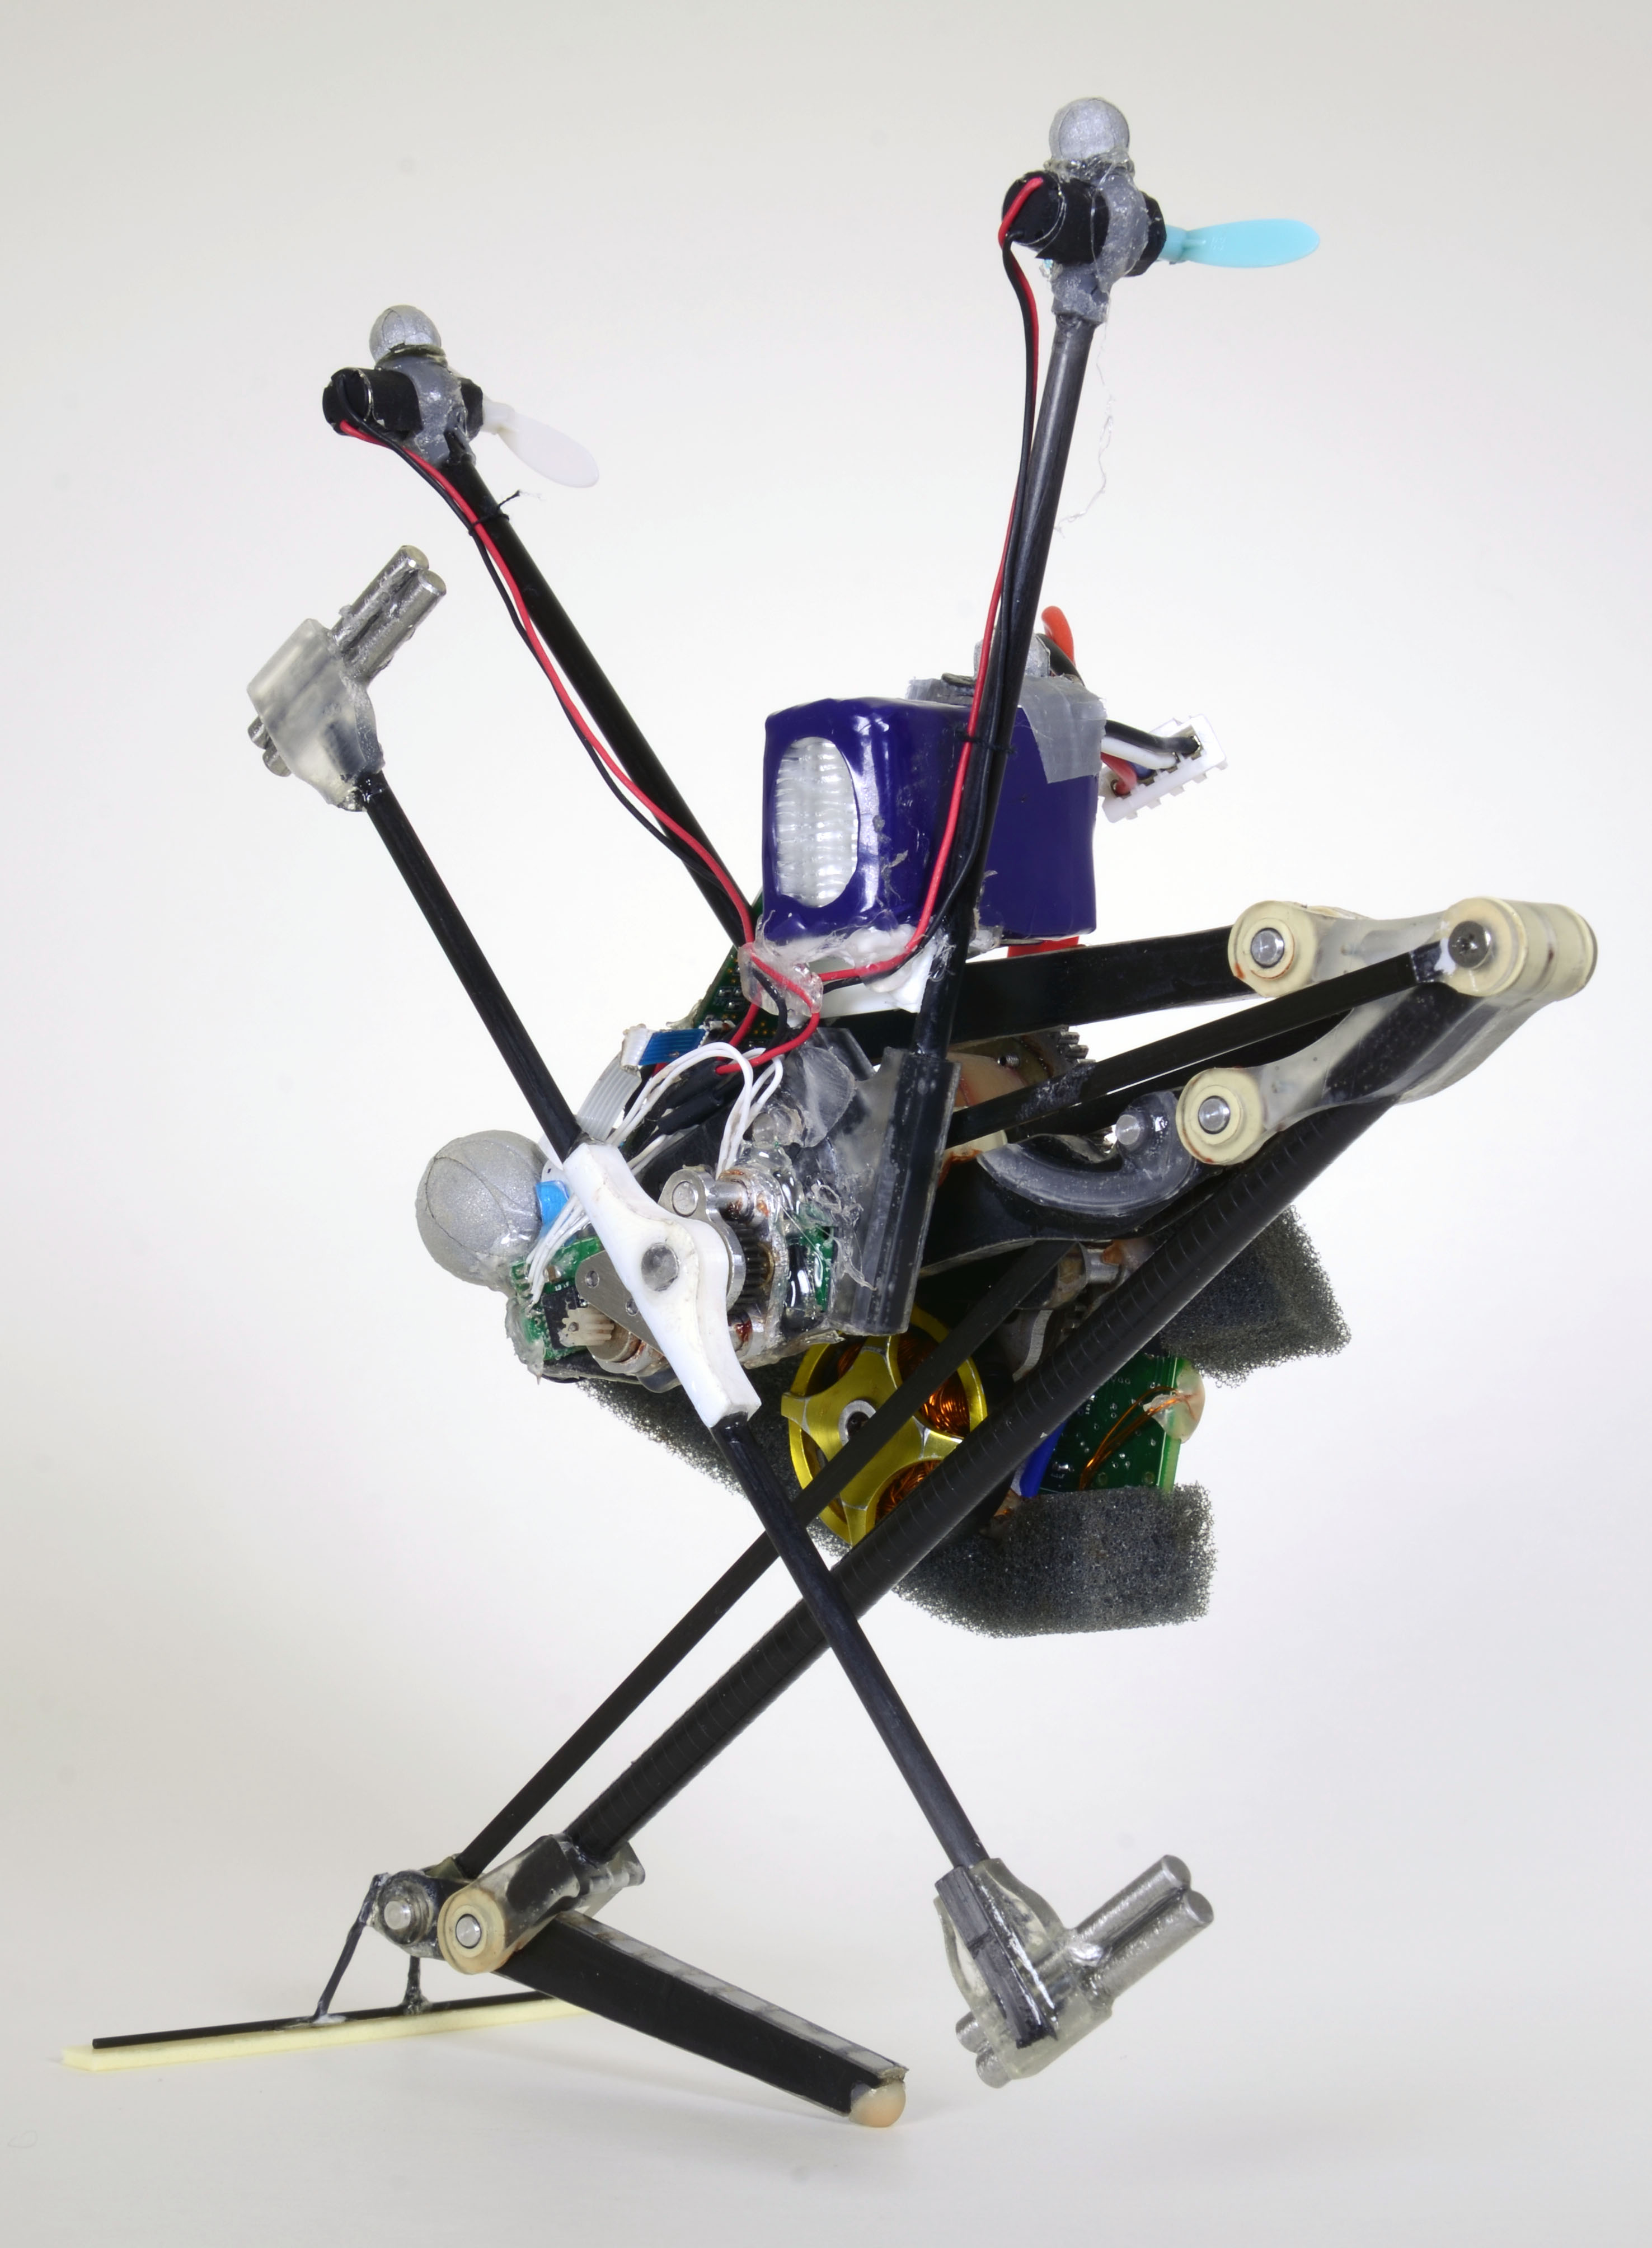
\includegraphics[height=8cm]{Salto-1P.jpg}
  \caption{Salto-1P机器人\cite{Salto1P}}
  \label{fig:salto-1p}
\end{figure}
Salto-1P的主要特点是通过SEA驱动结构实现了能量的存储,以保证跳跃瞬间的能量爆发。它可以每0.58秒进行一次高度1m的连续跳跃,这样的敏捷性无疑是惊人的。初代Salto\cite{Salto}腿长约15cm,重约100g,能量密度137W/kg,各方面指标已经接近或超越其设计之初的模仿对象————自然界的夜猴。为了实现精确控制,Salto身上装备了用于控制姿态的尾部,Salto-1P还配备了一对螺旋桨。前者在研究中只进行一次跳跃,而后者由于通过两个螺旋桨控制横滚(Roll)和偏航(Yaw),再加上尾部对俯仰(Pitch)的控制,实现了对空中身体姿态三个自由度的完全操控,因此可以做到连续跳跃。\\
对本项目的启示:
\begin{itemize}
  \item 本项目的弹跳部分设计参照了Salto腿部的机械模式,以提供有利于弹跳的机械增益曲线。
\end{itemize}
\subsection{Multimo-bat}
Multimo-bat多模态蝙蝠机器人是CMU机械系一位博士生2014年的作品。  
\begin{figure}[H]
  \centering
  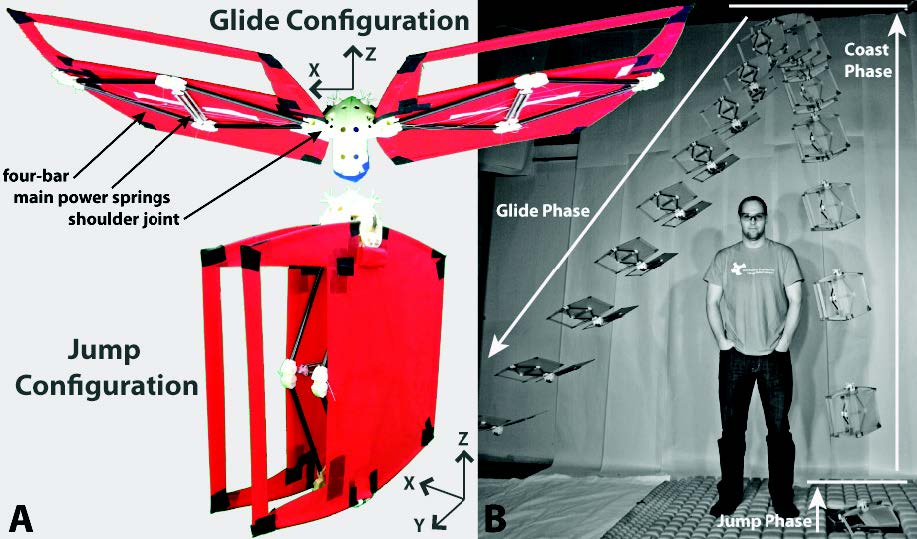
\includegraphics[height=8cm]{Multimo-bat.jpg}
  \caption{Multimo-bat机器人\cite{multimo}}
  \label{fig:multimo}
\end{figure}
如图\ref{fig:multimo}所示,该机器人主要拥有两个形态:跳跃态和滑翔态。其主要结构由身体和四连杆可折叠机翼构成。一个完整的跳跃滑翔运动过程如下:
\begin{enumerate}
  \item 图\ref{fig:multimo_struct}(a)中的主电机转动带动图中白线拉紧,此时四连杆收缩,电能转化为翼上弹簧的弹性势能存储起来。当收紧到一定程度后,触发内部结构的离合装置,充能完毕。
  \item 图\ref{fig:multimo_struct}(b)中的SMA丝通电发热收缩拉动离合器解锁,机翼快速弹回原位,弹簧释放能量,机器人跳起。
  \item 当机器人跳至最高点时,张开机翼,进入无动力滑翔模式。
\end{enumerate}
对本项目的启示:
\begin{itemize}
  \item 该项目的整体功能与本项目目标基本相同,其滑翔模式下通过控制重心来调整机翼攻角而不增加自由度的思想可以简化系统设计,增加鲁棒性。
\end{itemize}
\begin{figure}[h]
  \centering%
  \begin{subfigure}{3cm}
    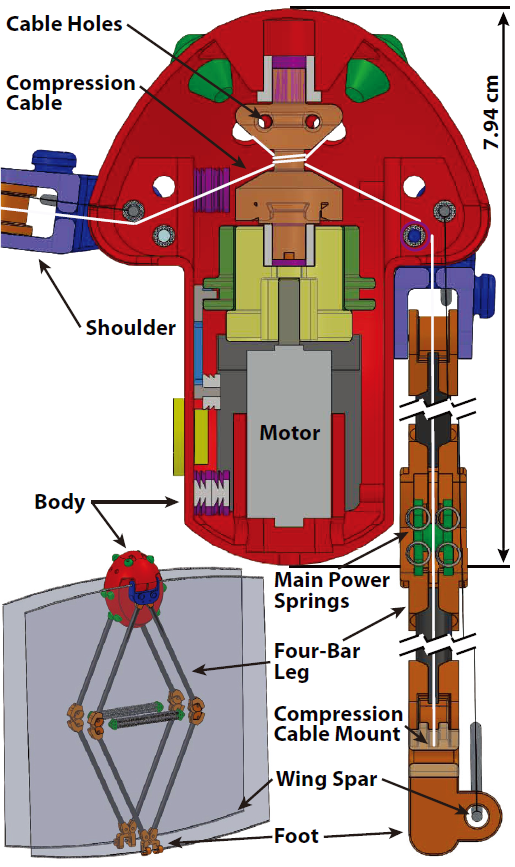
\includegraphics[height=10cm]{Multimo-bat_Structure.png}
    \caption{整体结构}
  \end{subfigure}%
  \hspace{10em}%
  \begin{subfigure}{0.5\textwidth}
    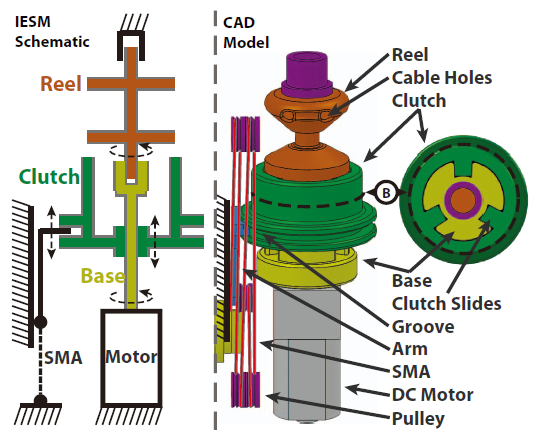
\includegraphics[height=8cm]{Multimo-bat_Structure2.png}
    \caption{离合器}
  \end{subfigure}
  \caption{Multimo-bat主要结构\cite{multimo}}
  \label{fig:multimo_struct}
\end{figure}

\subsection{EPFL Jumpglider}


对本文的启示:
\begin{itemize}
  \item 给出了跳跃滑翔模型的理论基础,以及最优化滑翔距离的方式。
\end{itemize}
% !TeX root = ../main.tex

\chapter{整体设计}
\label{cha:chapter02}
本项目选择把跳跃和滑翔分开作为两个独立的过程来分析与控制,用一个无刷电机驱动跳跃部分,用一个舵机控制机翼的开合。
\section{理论计算}
\label{sec:calculations}
取$g=9.8m/s^2$,预计机器人重量$m=200g$,跳跃高度$h=1m$,起跳电机做功时间$t=0.1s$,则机器人所需最小动能:
\begin{equation}
\label{equ:chap2:W_calc}
W_k=mgh
\end{equation}
二级齿轮减速器机械效率估计为$\eta=80\%$,则所需电机输出最小平均功率:
\begin{equation}
  \label{equ:chap2:P_calc}
  \bar{P}_{min}=\frac{W_k}{t·\eta}
  \end{equation}
解得:$$\bar{P}_{min}=24.5(W)$$
二级齿轮减速器减速比大约在10\sim30:1,设计中一次起跳输出级齿轮大约需要转半圈,取减速比20:1,则所需无刷电机转速:
$$\omega_{min}=0.5\times10\div t\times60=6000(rpm)$$
使用2S锂离子电池,额定电压$V=7.4V$,则所需最小电机KV值:
$$KV_{min}=\omega_{min}\div V=810(rpm/V)$$
一般来讲KV值越小无刷电机转矩越大,根据计算及机械需求考虑,选择了最大功率$P_{max}=168W$的朗宇X2305航模无刷电机,KV值$KV=1450$。\\
机器人起跳最小速度:
\begin{equation}
  \label{equ:chap2:v_calc}
  v=\sqrt{2gh}
  \end{equation}
根据动量定理:
\begin{equation}
  \label{equ:chap2:motion_principle}
  \bar{F}·t=m·v
  \end{equation}
解得所需平均力:$$\bar{F}=8.854(N)$$
航模用无刷电机的力矩数据不好获得,我们通过相同工作条件下的带螺旋桨升力进行估算,实际输出力只会更大。电机参数显示6000rpm时的升力等效质量约为$m_f=200\sim300g$,即经减速器输出的力为:$$F_min=m_{f,min}·g·20=39.2(N)>\bar{F}$$
此处还未考虑腿部连杆结构带来的机械增益,而其均值应>1,因此理论上输出力是足够支持跳跃的。
\section{元件选型}
\label{sec:components}
根据上述计算过程与现实考量,选择元件如表\ref{tab:bom}所示。
\begin{table}[htb]
  \centering
  \begin{minipage}[t]{0.8\linewidth}
  \caption{BOM表}
  \label{tab:bom}
    \begin{tabularx}{\linewidth}{lX}
      \toprule[1.5pt]
      {\heiti 元件名} & {\heiti 描述} \\\midrule[1pt]
      朗宇X2305无刷电机 & 外转子无刷电机,KV值1450 \\
      NanoPi Duo2 开发板 & 全志H3主控,运行Ubuntu 18.04\\
      FOC电机控制板 &  基于STSPINF0A方案的BLDC矢量控制 \\
      EMAX 2S航模锂电池 & 容量300mAh,质量为15g\\
      DS-S002M 4.3g数字舵机 & 用于控制机翼开合\\
      OV5640摄像头 & 500W像素,1080p@30fps,720p@60fps\\
      \bottomrule[1.5pt]
    \end{tabularx}
  \end{minipage}
\end{table}

\begin{figure}[H]
  \centering
  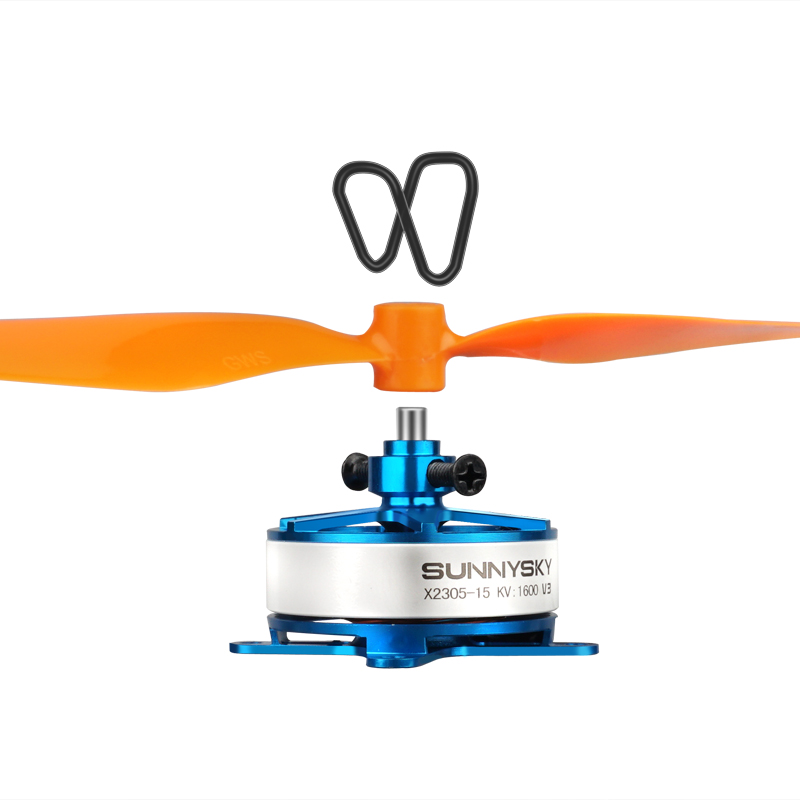
\includegraphics[height=10cm]{X2305.png}
  \caption{朗宇X2305无刷电机}
  \label{fig:X2305}
\end{figure}
\begin{figure}[H]
  \centering
  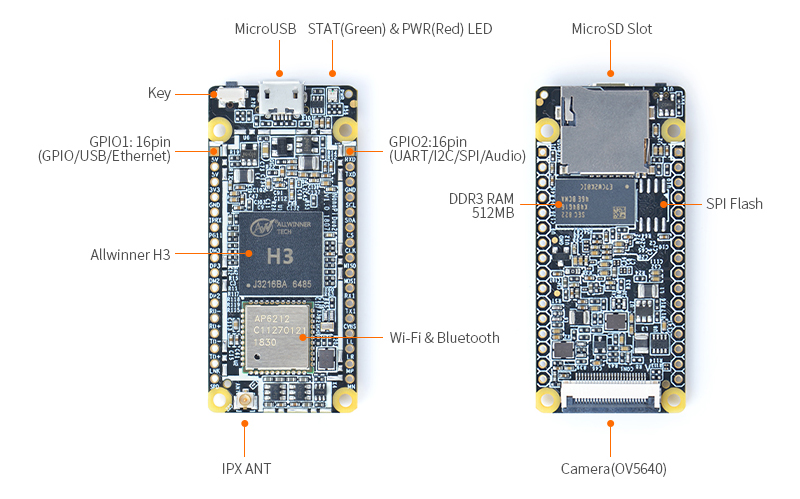
\includegraphics[height=10cm]{NanoPi-Duo2.jpg}
  \caption{NanoPi Duo2 开发板}
  \label{fig:Pi}
\end{figure}
\begin{figure}[H]
  \centering
  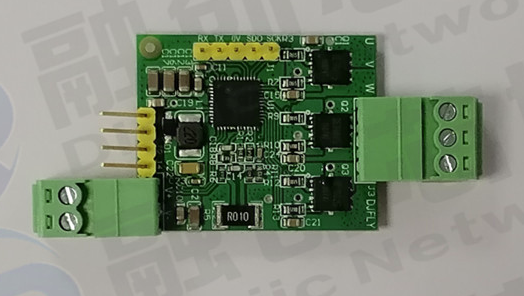
\includegraphics[height=7cm]{FOC.png}
  \caption{FOC电机控制板}
  \label{fig:FOC_board}
\end{figure}
\begin{figure}[H]
  \centering
  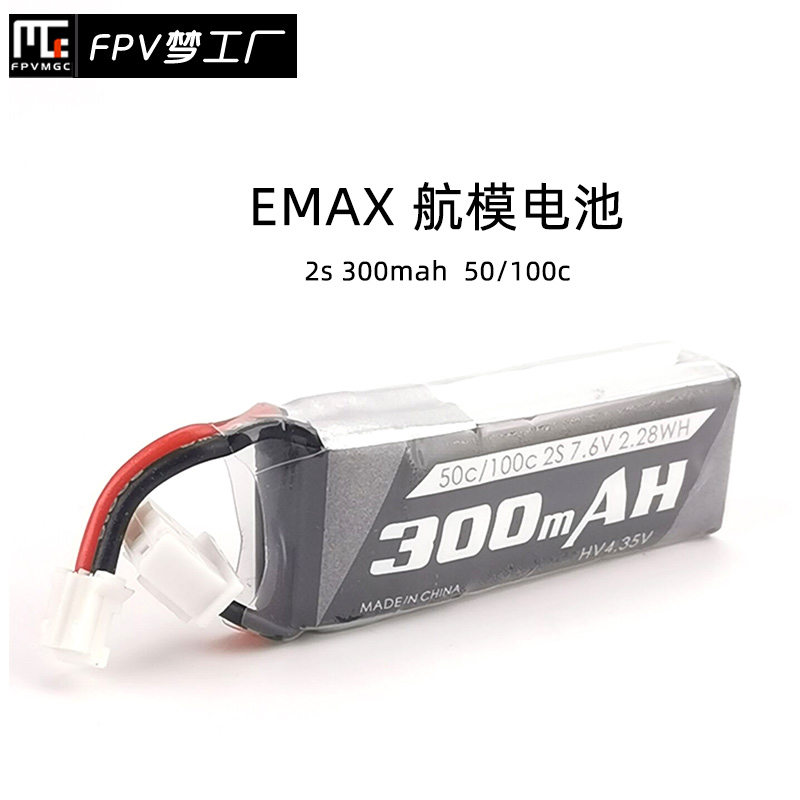
\includegraphics[height=10cm]{emax.jpg}
  \caption{EMAX 2S航模锂电池}
  \label{fig:emax}
\end{figure}
\begin{figure}[H]
  \centering
  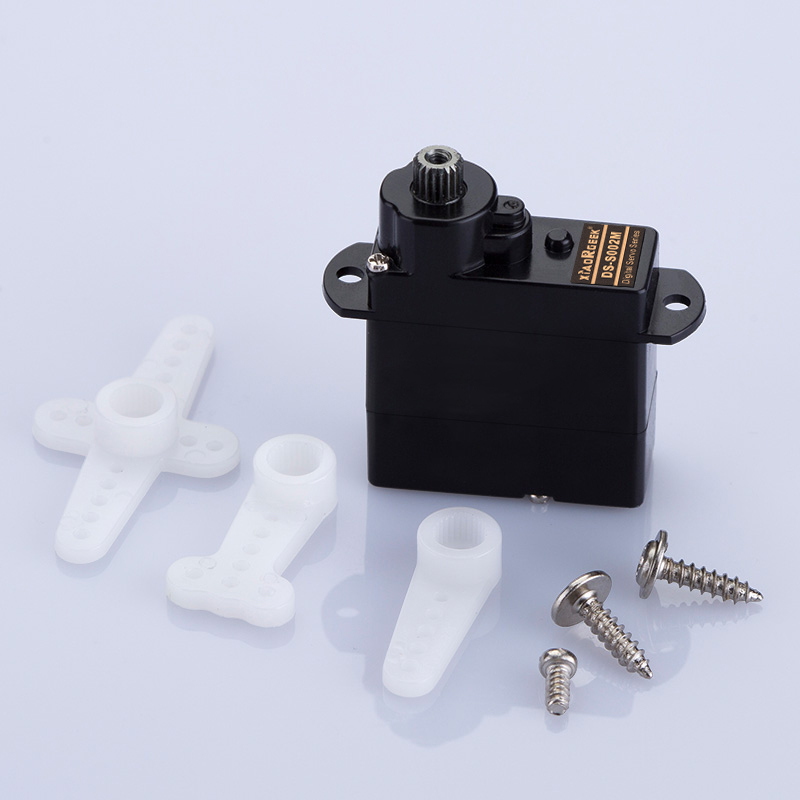
\includegraphics[height=10cm]{servo.jpg}
  \caption{DS-S002M 4.3g数字舵机}
  \label{fig:servo}
\end{figure}
\begin{figure}[H]
  \centering
  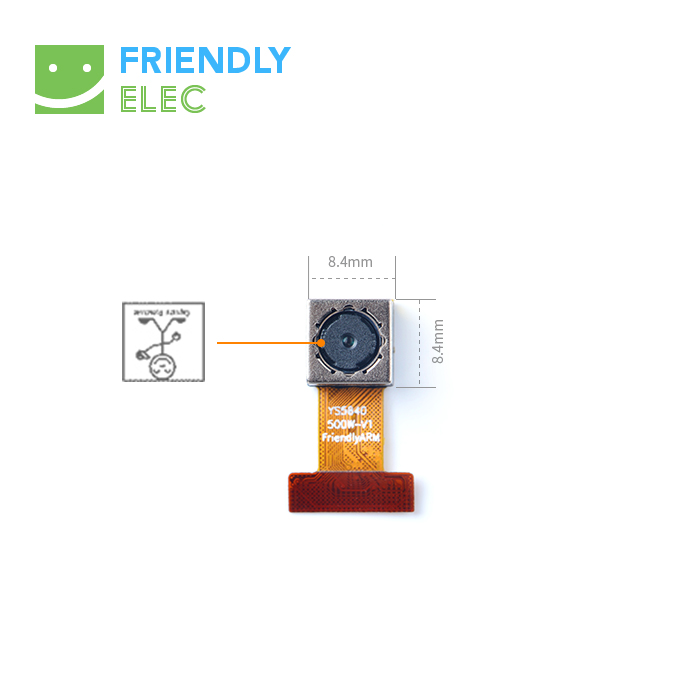
\includegraphics[height=10cm]{OV5640.jpg}
  \caption{OV5640摄像头}
  \label{fig:OV5640}
\end{figure}
\section{机械设计}
\label{sec:mechanical}
初步设计的机器人整体结构三维仿真图如下(螺丝等固定细节略去):
\begin{figure}[H]
  \centering
  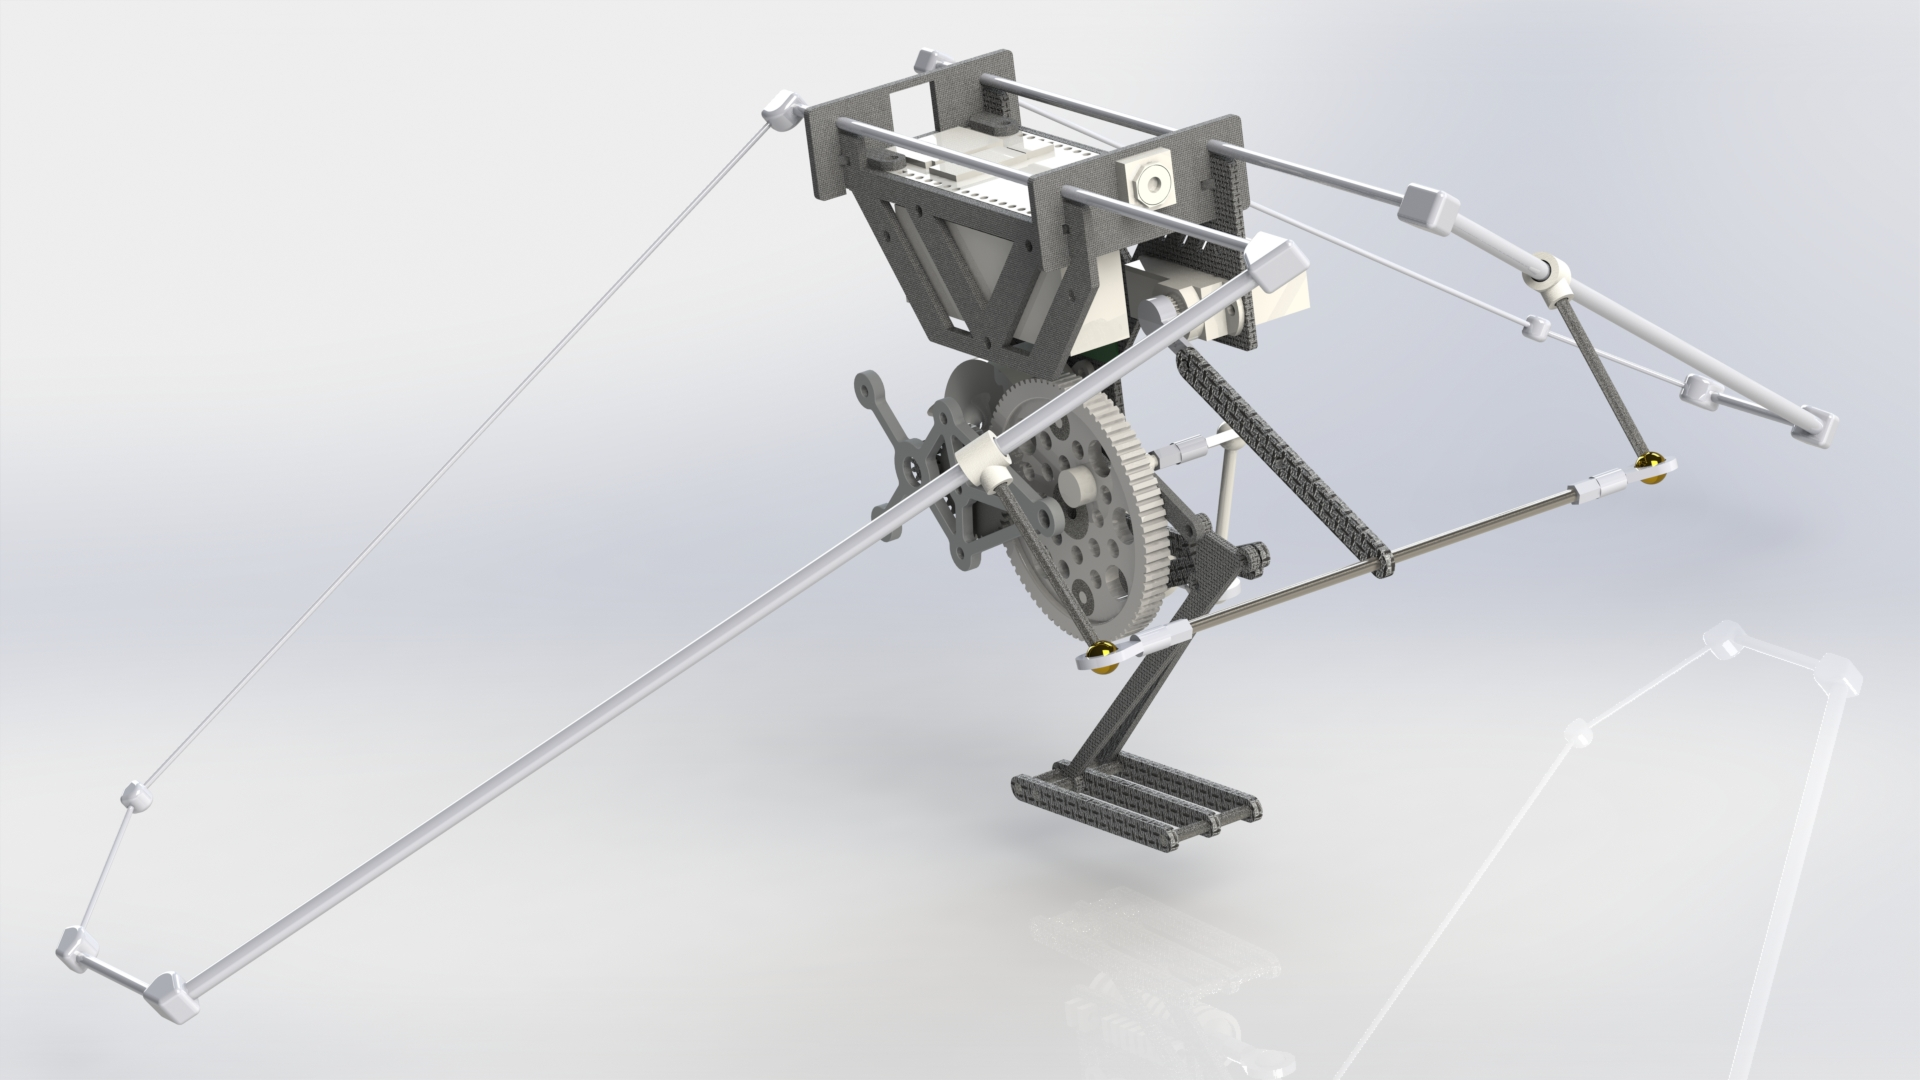
\includegraphics[height=8cm]{render2.jpg}
  \caption{整体结构渲染图}
  \label{fig:render_v1}
\end{figure}
\subsection{减速器设计}
设计目标为减速比20:1的两级齿轮减速器。考虑本项目实际尺寸,选用模数为0.5或0.6的齿轮较为合适。在市面上可直接买到的齿轮中,选择了0.5模数15齿的主轴齿轮,10/36齿的次级双层齿轮和80齿的末级齿轮。其中主轴齿轮材料为铜(粉末铸造),次级齿轮为铁基齿轮,而体积最大的末级齿轮采用了铝合金材质,兼顾了硬度与重量。

\begin{figure}[H]
  \centering
  \subcaptionbox{主轴齿轮\label{fig:cog1}}[4cm] 
    {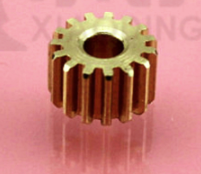
\includegraphics[height=3cm]{cog15.png}}
  \hspace{3em}
  \subcaptionbox{次级齿轮\label{fig:cog2}}[3cm]
      {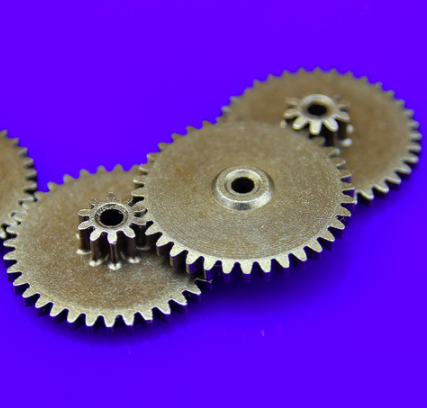
\includegraphics[height=3cm]{cog10_36.png}}
  \hspace{4em}
  \subcaptionbox{末级齿轮\label{fig:cog3}}
      {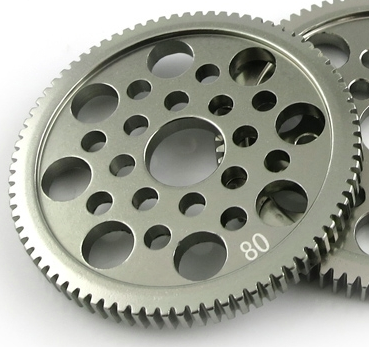
\includegraphics[height=3cm]{cog80.png}}
  \caption{齿轮的选择}
  \label{fig:cogs}

\end{figure}
实际减速比为:$$i=36\div15\times80\div10=19.2$$
据此我们设计出用于固定的减速器支架,选择铝合金材质CNC而成,保证连接强度的同时尽量减轻质量。设计图与实物图如图\ref{fig:retarder}所示,装配示意图如图\ref{fig:retarder_assembly}所示。
\begin{figure}[H]
  \centering
  \subcaptionbox{减速器模型\label{fig:retarder_model}}[7cm] 
    {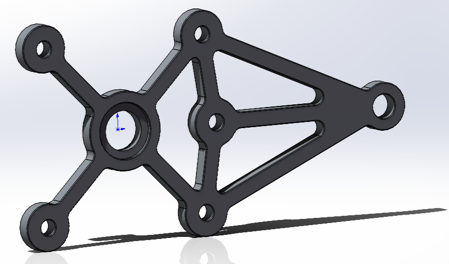
\includegraphics[height=4cm]{retarder_model.png}}
  \hspace{4em}
  \subcaptionbox{减速器实物\label{fig:retarder_real}}
      {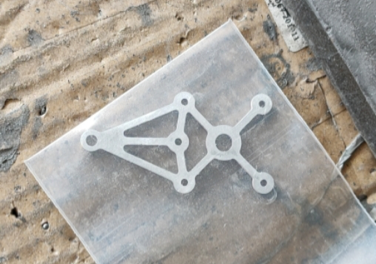
\includegraphics[height=4cm]{retarder_real.png}}
  \caption{减速器}
  \label{fig:retarder}
\end{figure}
\begin{figure}[H]
  \centering%
  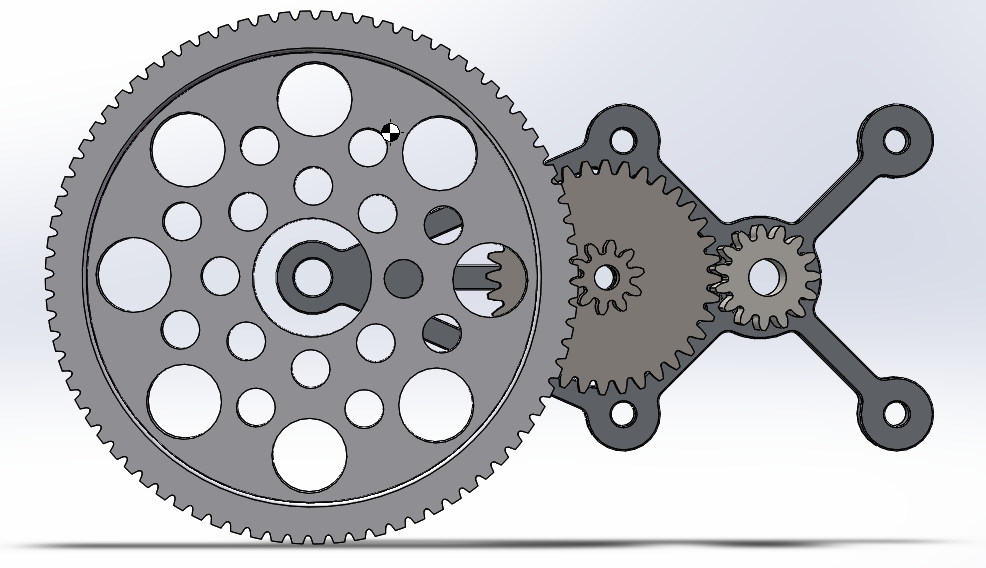
\includegraphics[height=8cm]{retarder_assembly.png}
  \caption{减速器装配图}
  \label{fig:retarder_assembly}
\end{figure}
\subsection{腿部设计}
参考Salto\cite{Salto}的腿部模型,此处实现了如图\ref{fig:2d_leg_fold}和图\ref{fig:2d_leg_stretch}所示的连杆结构。其中灰色圆为输出级齿轮,带动上部的曲柄-摇臂四连杆结构,同时四连杆摇臂为一凹四边形块,与机身相连的另一点在下部又组成了一个平行四边形四连杆,在输出级利用杠杆结构增大位移,实现触地端的较大速度,从而使身体跳起。虽然看上去略显复杂,但总体形态接近自然界大多数生物的腿部构造,这也从一个侧面反映了该结构的合理性。

\begin{figure}[H]
  \centering%
  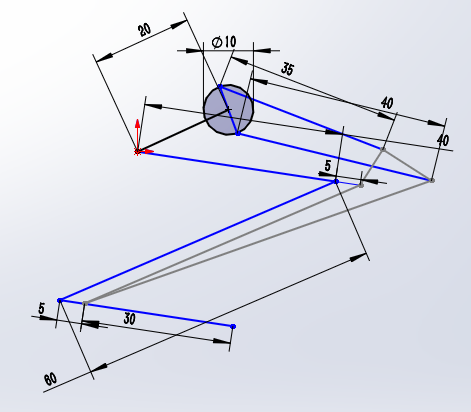
\includegraphics[height=6cm]{2d_leg_fold.png}
  \caption{起跳前准备姿势}
  \label{fig:2d_leg_fold}
\end{figure}
\begin{figure}[H]
  \centering%
  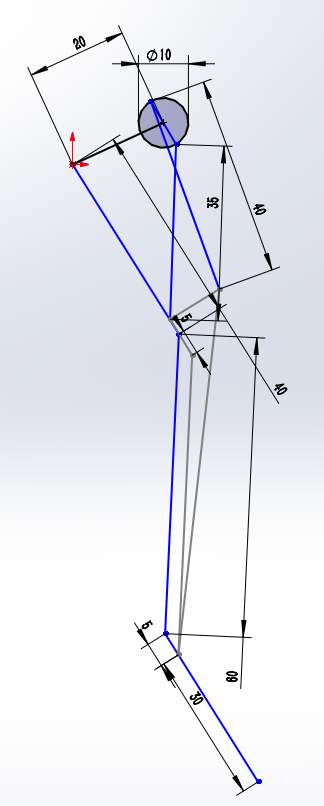
\includegraphics[height=11cm]{2d_leg_stretch.png}
  \caption{起跳后空中姿势}
  \label{fig:2d_leg_stretch}
\end{figure}

据此尺寸在SolidWorks中设计出三维模型,装配示意图如图\ref{fig:3d_leg}所示。
\begin{figure}[H]
  \centering%
  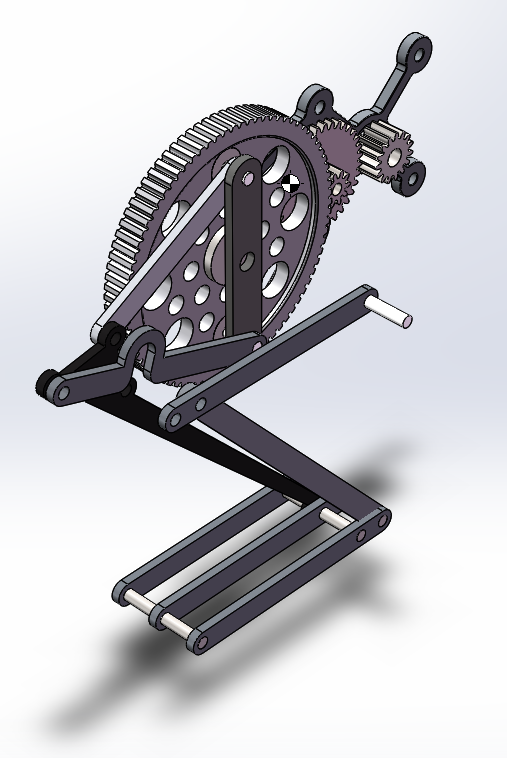
\includegraphics[height=8cm]{3d_leg.png}
  \caption{腿部装配图}
  \label{fig:3d_leg}
\end{figure}

\subsection{机翼设计}
\label{sec:wings}
采用蝴蝶式\cite{EPFL}折叠机翼设计,利用一个小舵机带动两片机翼的同步开合。为了降低机翼质量,采用碳纤维骨架与蒙皮的形式,骨架由碳纤维杆与3D打印的接头组成,翼面材料使用潍坊风筝布料,以保证强度与抗老化性。机翼部分设计模型如图\ref{fig:wings_mechanism}所示。
\begin{figure}[H]
  \centering%
  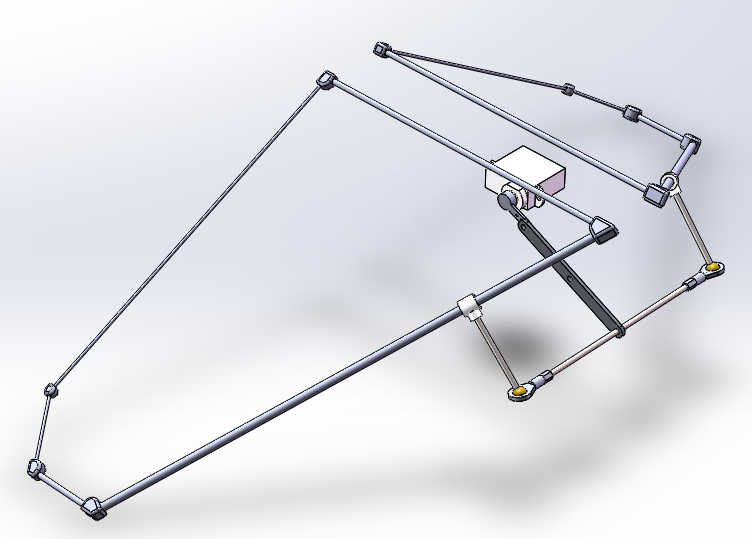
\includegraphics[height=8cm]{wings_mechanism.png}
  \caption{机翼原理图}
  \label{fig:wings_mechanism}
\end{figure}

\subsection{机身设计}
机身设计目标:实现腿、机翼和其他元件的可靠连接。
\begin{figure}[H]
  \centering%
  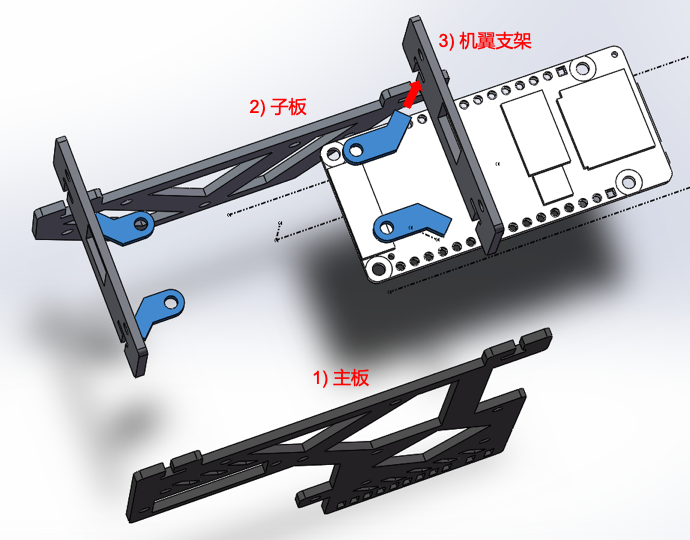
\includegraphics[height=10cm]{mt_exploded_marked.png}
  \caption{榫卯结构爆炸视图}
  \label{fig:mt_exploded}
\end{figure}
为了降低制造难度,我们希望所有的设计都尽可能是平面的。而在三维世界中实现二维平面物体之间的连接,就要使用一些连接结构。为了降低装配难度及提高鲁棒性(在如此小的体积上拧螺丝也并非易事),在机身主板与各子板之间的连接设计上参考了我国古代人民智慧的结晶——榫卯结构。如图\ref{fig:mt_exploded}所示,蓝色楔子即为榫头,2号子板与3号机翼支架之间的空隙构成了榫眼,红色箭头标出了楔子的运动方向。装配好的结构如图\ref{fig:mt_assembled}所示。此时四角的楔子与主控板以螺丝螺母紧固,使得三个方向的平面得以可靠连接,同时并未使用除电路板四个螺丝孔以外的任何螺丝安装,实现了简洁而高效的机械结构。
\begin{figure}[H]
  \centering
  {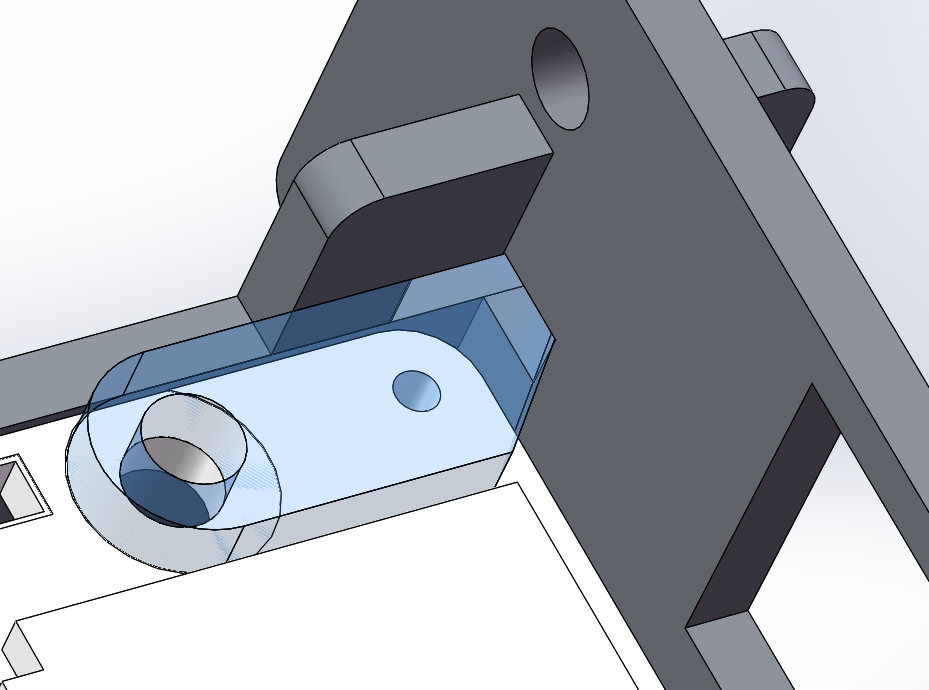
\includegraphics[height=10cm]{mt_zoom.png}}
  \caption{榫卯连接处透视图}
  \label{fig:mt_zoom}
\end{figure}
\begin{figure}[H]
  \centering
  {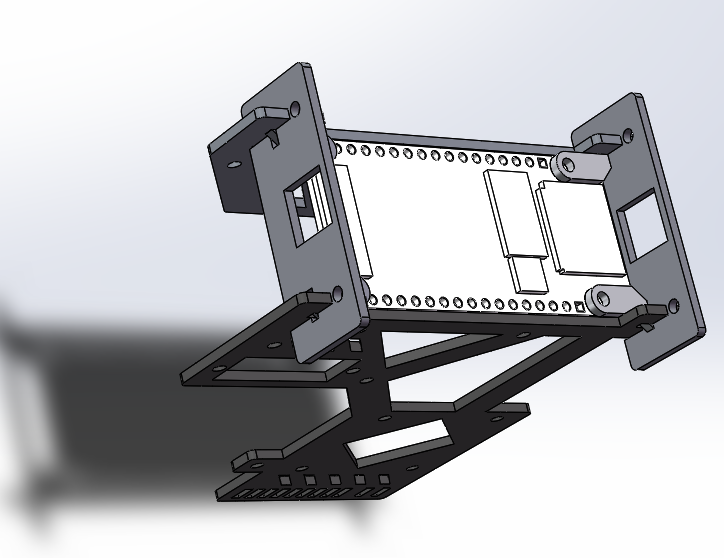
\includegraphics[height=10cm]{mt_assembled.png}}
  \caption{主板、子板、机翼支架和电路板装配完成}
  \label{fig:mt_assembled}
\end{figure}
\subsection{磁助力装置}
为了增加起跳时的爆发力,设计了如图\ref{fig:magnet_fold}、\ref{fig:magnet_jump}所示的磁助力装置。机器人下蹲时电机需要克服磁力做功,相当于将能量存储到磁场中。
\begin{figure}[H]
  \centering
  {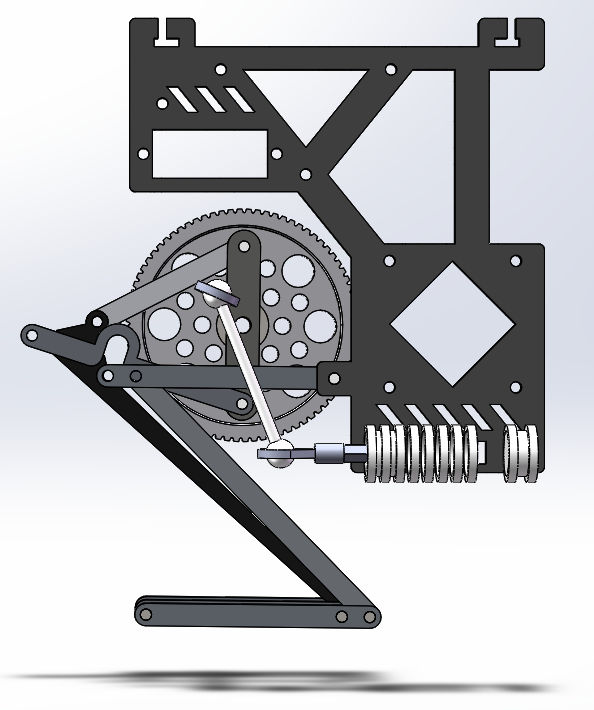
\includegraphics[height=7cm]{magnet_fold.png}}
  \caption{折叠状态磁场储能}
  \label{fig:magnet_fold}
\end{figure}
\begin{figure}[H]
  \centering
  {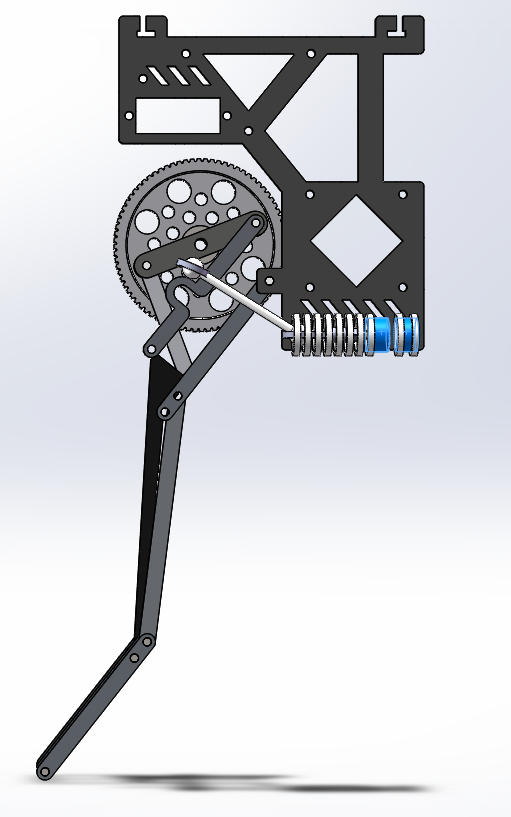
\includegraphics[height=10cm]{magnet_jump.png}}
  \caption{跳跃时磁场做功}
  \label{fig:magnet_jump}
\end{figure}
\subsection{整体装配图}
机身全部装配图如下:
\begin{figure}[H]
  \centering
  {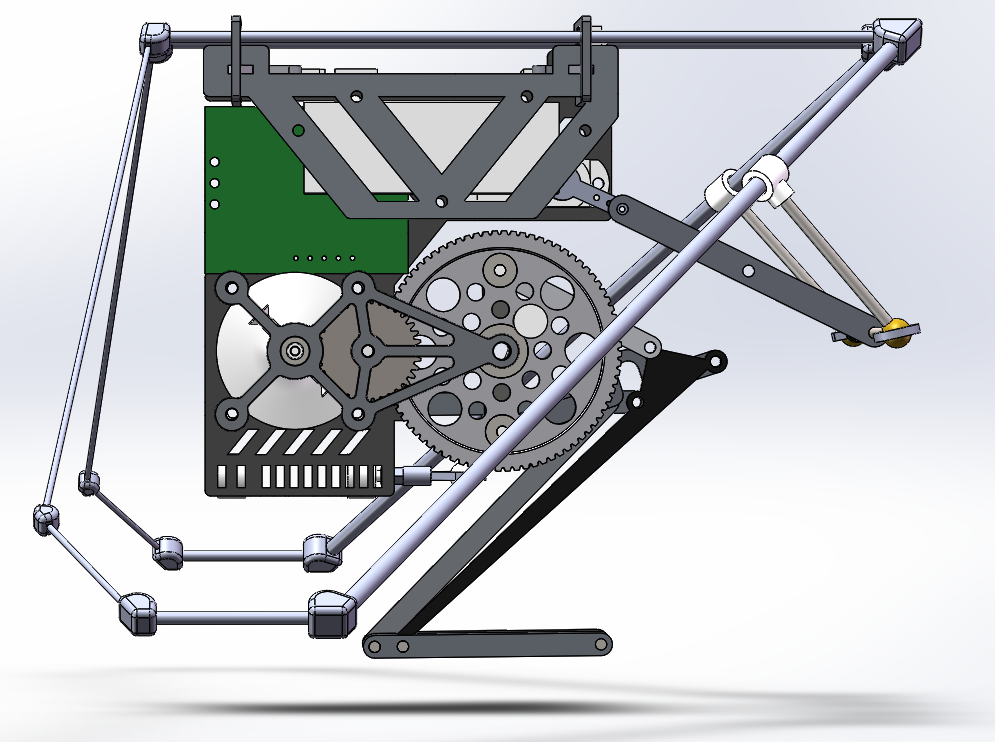
\includegraphics[height=10cm]{left.png}}
  \caption{左视图}
  \label{fig:left}
\end{figure}
\begin{figure}[H]
  \centering
  {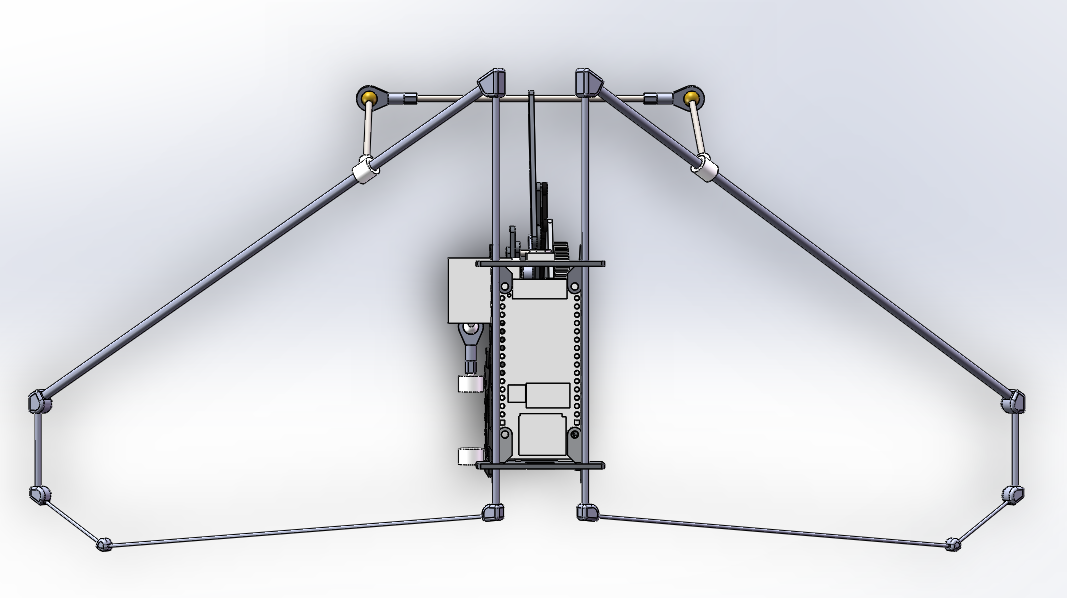
\includegraphics[height=8cm]{up.png}}
  \caption{俯视图}
  \label{fig:up}
\end{figure}
\begin{figure}[H]
  \centering
  {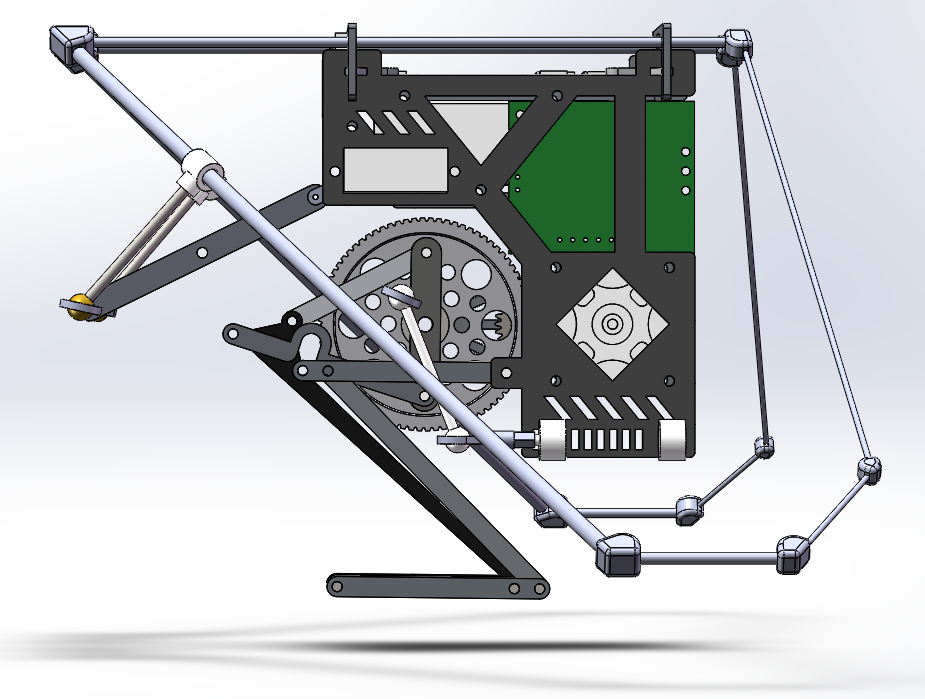
\includegraphics[height=11cm]{right.png}}
  \caption{右视图}
  \label{fig:right}
\end{figure}
\begin{figure}[H]
  \centering
  {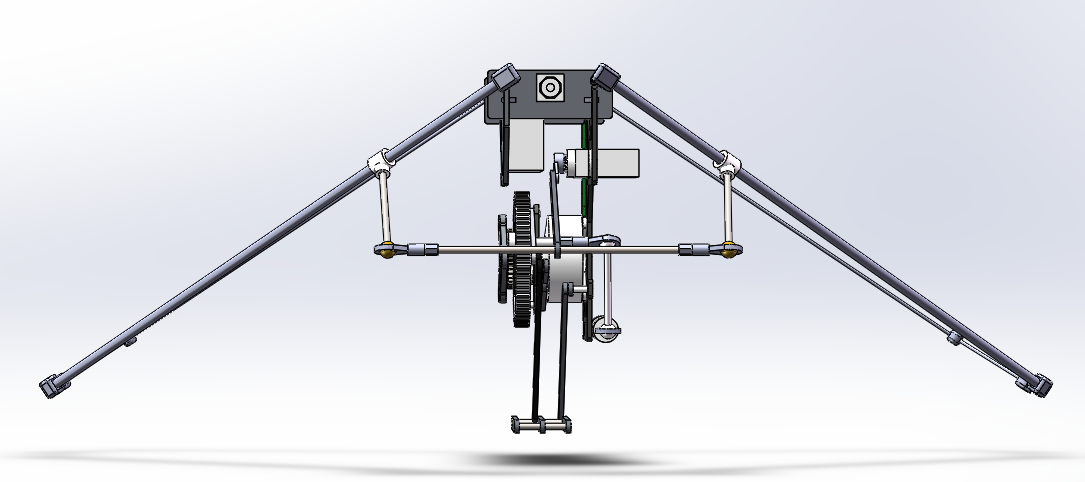
\includegraphics[height=7cm]{front.png}}
  \caption{正视图}
  \label{fig:front}
\end{figure}
\begin{figure}[H]
  \centering
  {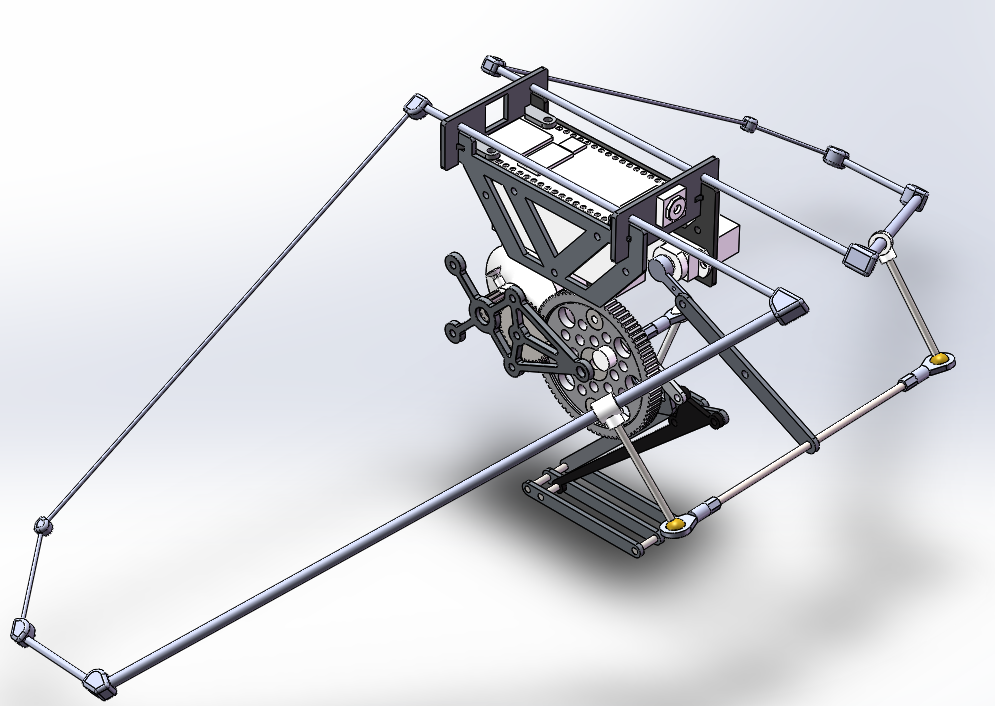
\includegraphics[height=10cm]{leftup.png}}
  \caption{左上等轴测视图}
  \label{fig:leftup}
\end{figure}
\begin{figure}[H]
  \centering
  {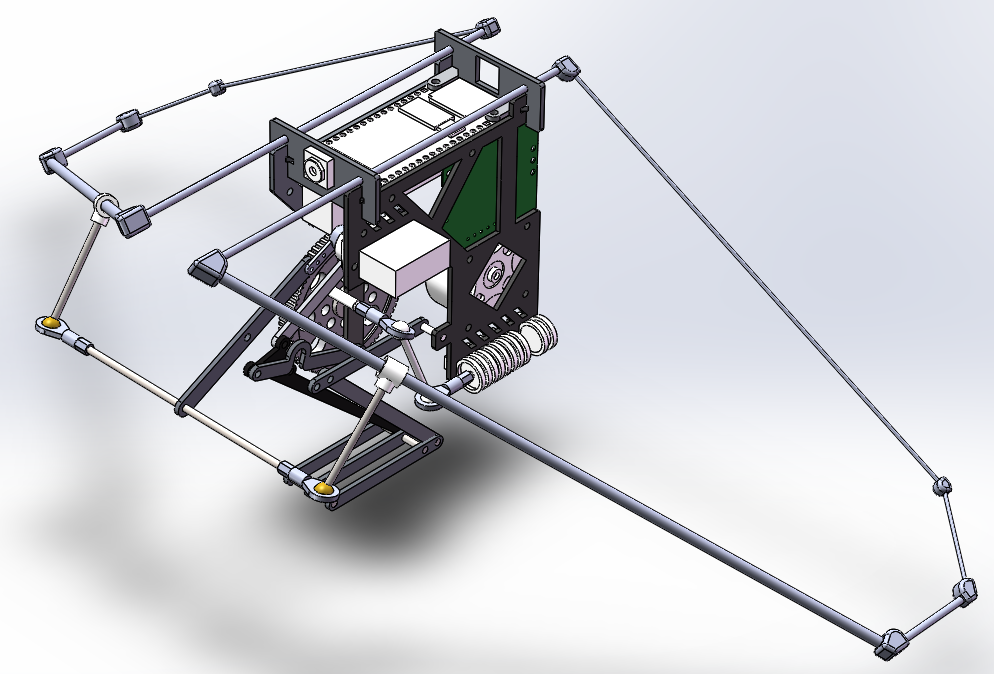
\includegraphics[height=10cm]{rightup.png}}
  \caption{右上等轴测视图}
  \label{fig:rightup}
\end{figure}
\section{嵌入式系统}
电路部分系统架构如图\ref{fig:system_architecture}所示。电源部分,2S锂电池直接接入FOC控制板,FOC控制板上自带稳压芯片提供STSPIN32F0A芯片所需的3.3V;而同时并联一个5V稳压模块,给主控板NanoPi供电。主控板通过UART与FOC控制板通讯,进而控制电机。同时主控板还直接通过PWM控制舵机位置,并通过MIPI接口连接OV5640摄像头,通过Wi-Fi传回实时图像数据。上位机也通过Wi-Fi向机器人发送指令。
\begin{figure}[H]
  \centering
  {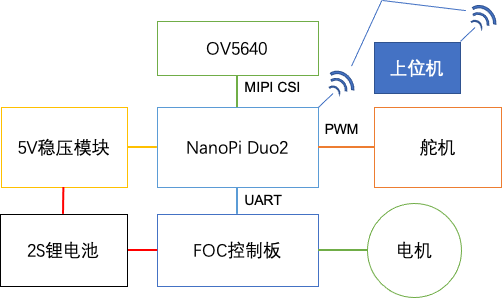
\includegraphics[height=5cm]{system_architecture.png}}
  \caption{系统架构}
  \label{fig:system_architecture}
\end{figure}
\subsection{控制算法}
电机控制部分主要使用了工业上成熟的FOC矢量控制技术\cite{FOC}。FOC的核心思想是使定子电流的磁场始终与转子的磁场正交,从而始终保持扭矩最大。因此其数学基础就是三相坐标系与直角坐标系之间的坐标变换,以及控制理论中的PID控制。而实际情况远比这个简单的理想模型要复杂,因此本项目选择站在前人的肩膀上,使用来自意法半导体的成熟的ST FOC电机库\cite{MCSDK},实现对电机的精确控制。
\begin{figure}[H]
  \centering
  {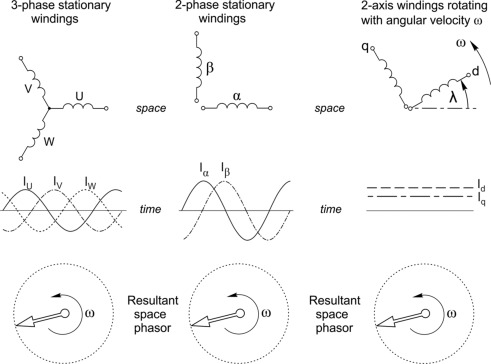
\includegraphics[height=8cm]{FOC.jpg}}
  \caption{FOC电流坐标变换\cite{FOC}}
  \label{fig:FOC}
\end{figure}
如图\ref{fig:FOC}所示,以$\alpha$,$\beta$所在轴建立直角坐标系,投影可得:
$$
  \left\{
  \begin{aligned}
  I_\alpha & = &I_U-cos(\frac{\pi}{3})I_V-cos(\frac{\pi}{3})I_W \\
  I_\beta  & = &sin(\frac{\pi}{3})I_V-sin(\frac{\pi}{3})I_W
  \end{aligned}
  \right.
$$
即:
\begin{equation}
  \label{equ:chap2:clark}
  \left[ \begin{array}{c}
  I_\alpha \\
  I_\beta
  \end{array}
  \right]=K\left[ 
    \begin{array}{ccc}
    1 & -\frac{1}{2} & -\frac{1}{2}\\
    0 & \frac{\sqrt{3}}{2} & -\frac{\sqrt{3}}{2}   
    \end{array}
    \right]\left[ \begin{array}{c}
      I_U \\
      I_V \\
      I_W
      \end{array}
      \right]
\end{equation}
式\ref{equ:chap2:clark}被称为Clark变换。自然地,有:
\begin{equation}
  \label{equ:chap2:clark_inv}
  \left[ \begin{array}{c}
    I_U \\
    I_V \\
    I_W
    \end{array}
    \right]=K\prime\left[ 
    \begin{array}{cc}
    1 & 0 \\
    -\frac{1}{2} & \frac{\sqrt{3}}{2} \\
    -\frac{1}{2} & -\frac{\sqrt{3}}{2}   
    \end{array}
    \right]\left[ \begin{array}{c}
      I_\alpha \\
      I_\beta
      \end{array}
      \right]
\end{equation}
式\ref{equ:chap2:clark_inv}被称为Clark逆变换。Clark正逆变换完成了交流三相坐标系与直角坐标系之间电流的转换,是磁场定向控制的基础。而在图\ref{fig:FOC}的第二部分到第三部分,要完成从静止坐标系到旋转坐标系的变换。由几何关系有:
$$
  \left\{
  \begin{aligned}
  I_d & = & I_\alpha cos(\lambda)+I_\beta sin(\lambda) \\
  I_q & = & -I_\alpha sin(\lambda)+I_\beta cos(\lambda)
  \end{aligned}
  \right.
$$
即:
\begin{equation}
  \label{equ:chap2:park}
  \left[ \begin{array}{c}
  I_d \\
  I_q
  \end{array}
  \right]=\left[ 
    \begin{array}{cc}
    cos(\lambda) & sin(\lambda)\\
    -sin(\lambda) & cos(\lambda)   
    \end{array}
    \right]\left[ \begin{array}{c}
      I_\alpha \\
      I_\beta
      \end{array}
      \right]
\end{equation}
式\ref{equ:chap2:park}被称为Park变换。易得其逆变换公式:
\begin{equation}
  \label{equ:chap2:park_inv}
  \left[ \begin{array}{c}
  I_\alpha \\
  I_\beta
  \end{array}
  \right]=\left[ 
    \begin{array}{cc}
    cos(\lambda) & -sin(\lambda)\\
    sin(\lambda) & cos(\lambda)   
    \end{array}
    \right]\left[ \begin{array}{c}
      I_d \\
      I_q
      \end{array}
      \right]
\end{equation}
而在嵌入式系统上,更注重算法执行的效率,因此三角函数运算多由查表获得。
\subsection{串口通信协议}
ST MotorControl SDK\cite{MCSDK}提供了如图\ref{fig:MCSDK_UI}所示的功能强大的UI,但却并未提供通信协议细节。好在这是一个开源项目,通过阅读SDK源代码,得到串口通信协议如下:
\begin{figure}[h]
  \centering
  {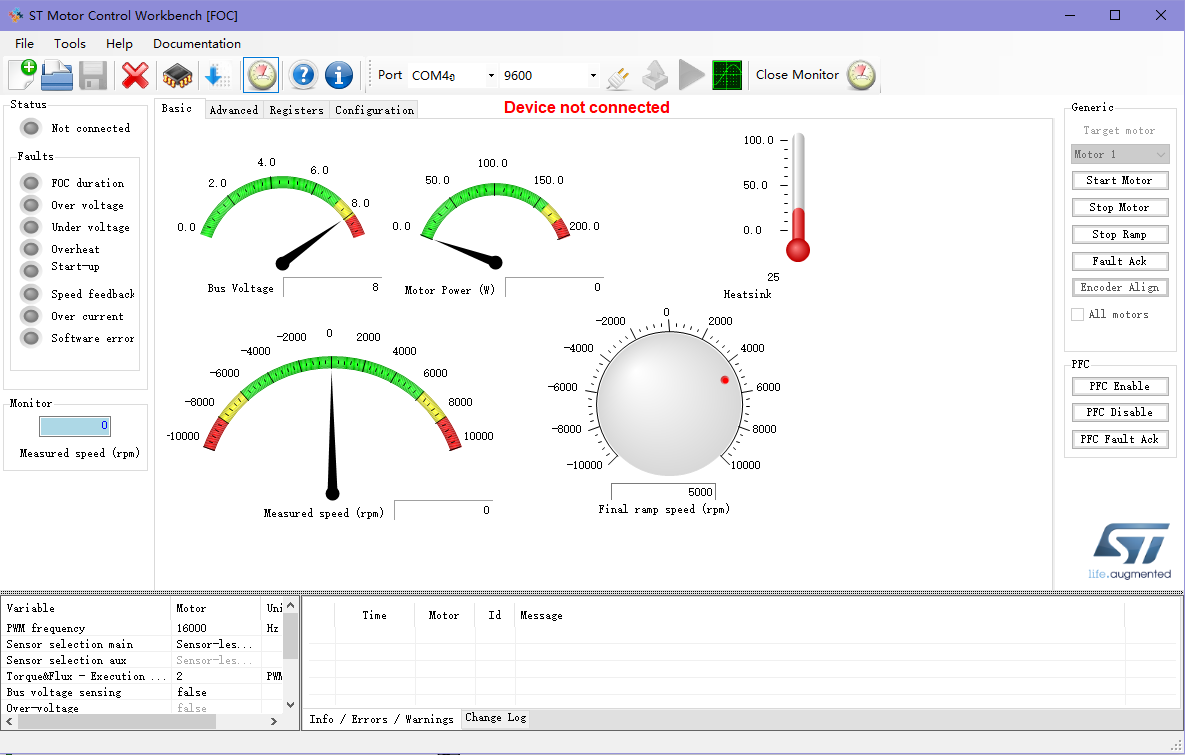
\includegraphics[height=10cm]{MCSDK_UI.png}}
  \caption{MotorControl Workbench上位机\cite{MCSDK}}
  \label{fig:MCSDK_UI}
\end{figure}
\begin{table}[htb]
  \centering
  \begin{minipage}[t]{0.8\linewidth}
  \caption{通信协议(默认波特率9600bps)}
  \label{tab:UART_protocol}
    \begin{tabularx}{\linewidth}{llX}
      \toprule[1.5pt]
      {\heiti 代号} & {\heiti 长度(字节)} & {\heiti 描述} \\\midrule[1pt]
      Code & 1 & 操作码,标识当前数据包的功能 \\
      Size & 1 & 传输负载长度 \\
      Payload & Size & 负载,用于传输命令参数 \\
      CRC & 1 & 校验位\\
      \bottomrule[1.5pt]
    \end{tabularx}
  \end{minipage}
\end{table}
其中校验位的计算方式为将数据包中CRC之前的所有位求和,用一个无符号16位整型变量存储,再把得到的结果的高8位右移8位与低8位相加,得到的结果存入一个8位无符号整型变量(也就是说在最后这步加法中无视溢出)。平心而论,这个操作只能说是魔改的求和校验,并不属于CRC,因为真正的CRC是有纠错能力的,而这个魔改的求和校验码只具有检错能力,因此这个变量名取Parity更为妥当,此处保留了源代码中的变量名。但在这种简单的串口通信中也无须纠错,误码重传代价不大,可以接受。
\subsection{通信系统}
本项目的主要通信框架为ROS\cite{ROS}(Robot Operating System,机器人操作系统)。与Ubuntu 18.04系统对应的ROS版本是ROS Melodic。ROS是一套发布-订阅机制的通信框架,需要一台主机运行roscore作为服务器,其他主机连接到这台服务器来发布和订阅消息。在本项目中主要通过ROS回传摄像头图像数据,可以很方便的在ROS中配置摄像头参数。
\begin{figure}[H]
  \centering
  {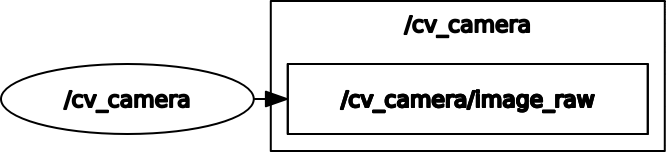
\includegraphics[height=3cm]{rosgraph.png}}
  \caption{ROS节点消息图}
  \label{fig:rosgraph}
\end{figure}


% 其它部分
\backmatter

%% 本科生要求的几个索引。
\listoffigures    % 插图索引
\listoftables     % 表格索引
\listofequations  % 公式索引

% 参考文献
\bibliographystyle{thuthesis-numeric}      % 顺序编码制
% \bibliographystyle{thuthesis-author-year}  % 著者-出版年制
% \bibliographystyle{thuthesis-bachelor}     % 本科生参考文献的著录格式
\bibliography{ref/refs}

% 致谢
% !TeX root = ../main.tex

\begin{acknowledgements}
  衷心感谢导师 xxx 教授和物理系 xxx 副教授对本人的精心指导。他们的言传身教将使
  我终生受益。

  在美国麻省理工学院化学系进行九个月的合作研究期间,承蒙 xxx 教授热心指导与帮助,不
  胜感激。感谢 xx 实验室主任 xx 教授,以及实验室全体老师和同学们的热情帮助和支
  持!本课题承蒙国家自然科学基金资助,特此致谢。

  感谢 \LaTeX{} 和 \thuthesis,帮我节省了不少时间。
\end{acknowledgements}


% 声明
\statement

% 附录
\appendix
% !TeX root = ../main.tex

\begin{survey}
\label{cha:survey}

\title{Title of the Survey}
\maketitle

写出至少 5000 外文印刷字符的调研阅读报告或者书面翻译 1-2 篇(不少于 2 万外文印刷符)。

It is impossible to cover in a single chapter every concept of mathematical
programming.\cite{tex} This chapter introduces only the basic concepts and techniques of
mathematical programming such that readers gain an understanding of them
throughout the book\cite{abrahams99tex,salomon1995advanced}.


\section{Single-Objective Programming}
The general form of single-objective programming (SOP) is written
as follows,
\begin{equation*} % 如果附录中的公式不想让它出现在公式索引中,那就请
                             % 用 equation*
\left\{\begin{array}{l}
\max \,\,f(x)\\[0.1 cm]
\mbox{subject to:} \\ [0.1 cm]
\qquad g_j(x)\le 0,\quad j=1,2,\cdots,p
\end{array}\right.
\end{equation*}
which maximizes a real-valued function $f$ of
$x=(x_1,x_2,\cdots,x_n)$ subject to a set of constraints.

\newcommand\Real{\mathbf{R}}
\newtheorem{mpdef}{Definition}[chapter]
\begin{mpdef}
In SOP, we call $x$ a decision vector, and
$x_1,x_2,\cdots,x_n$ decision variables. The function
$f$ is called the objective function. The set
\begin{equation*}
S=\left\{x\in\Real^n\bigm|g_j(x)\le 0,\,j=1,2,\cdots,p\right\}
\end{equation*}
is called the feasible set. An element $x$ in $S$ is called a
feasible solution.
\end{mpdef}

\newtheorem{mpdefop}[mpdef]{Definition}
\begin{mpdefop}
A feasible solution $x^*$ is called the optimal
solution of SOP if and only if
\begin{equation}
f(x^*)\ge f(x)
\end{equation}
for any feasible solution $x$.
\end{mpdefop}

One of the outstanding contributions to mathematical programming was known as
the Kuhn-Tucker conditions\ref{eq:ktc}. In order to introduce them, let us give
some definitions. An inequality constraint $g_j(x)\le 0$ is said to be active at
a point $x^*$ if $g_j(x^*)=0$. A point $x^*$ satisfying $g_j(x^*)\le 0$ is said
to be regular if the gradient vectors $\nabla g_j(x)$ of all active constraints
are linearly independent.

Let $x^*$ be a regular point of the constraints of SOP and assume that all the
functions $f(x)$ and $g_j(x),j=1,2,\cdots,p$ are differentiable. If $x^*$ is a
local optimal solution, then there exist Lagrange multipliers
$\lambda_j,j=1,2,\cdots,p$ such that the following Kuhn-Tucker conditions hold,
\begin{equation}
\label{eq:ktc}
\left\{\begin{array}{l}
    \nabla f(x^*)-\sum\limits_{j=1}^p\lambda_j\nabla g_j(x^*)=0\\[0.3cm]
    \lambda_jg_j(x^*)=0,\quad j=1,2,\cdots,p\\[0.2cm]
    \lambda_j\ge 0,\quad j=1,2,\cdots,p.
\end{array}\right.
\end{equation}
If all the functions $f(x)$ and $g_j(x),j=1,2,\cdots,p$ are convex and
differentiable, and the point $x^*$ satisfies the Kuhn-Tucker conditions
(\ref{eq:ktc}), then it has been proved that the point $x^*$ is a global optimal
solution of SOP.

\subsection{Linear Programming}
\label{sec:lp}

If the functions $f(x),g_j(x),j=1,2,\cdots,p$ are all linear, then SOP is called
a {\em linear programming}.

The feasible set of linear is always convex. A point $x$ is called an extreme
point of convex set $S$ if $x\in S$ and $x$ cannot be expressed as a convex
combination of two points in $S$. It has been shown that the optimal solution to
linear programming corresponds to an extreme point of its feasible set provided
that the feasible set $S$ is bounded. This fact is the basis of the {\em simplex
  algorithm} which was developed by Dantzig as a very efficient method for
solving linear programming.
\begin{table}[ht]
\centering
  \centering
  \caption*{Table~1\hskip1em This is an example for manually numbered table, which
    would not appear in the list of tables}
  \label{tab:badtabular2}
  \begin{tabular}[c]{|m{1.5cm}|c|c|c|c|c|c|}\hline
    \multicolumn{2}{|c|}{Network Topology} & \# of nodes &
    \multicolumn{3}{c|}{\# of clients} & Server \\\hline
    GT-ITM & Waxman Transit-Stub & 600 &
    \multirow{2}{2em}{2\%}&
    \multirow{2}{2em}{10\%}&
    \multirow{2}{2em}{50\%}&
    \multirow{2}{1.2in}{Max. Connectivity}\\\cline{1-3}
    \multicolumn{2}{|c|}{Inet-2.1} & 6000 & & & &\\\hline
    \multirow{2}{1.5cm}{Xue} & Rui  & Ni &\multicolumn{4}{c|}{\multirow{2}*{\thuthesis}}\\\cline{2-3}
    & \multicolumn{2}{c|}{ABCDEF} &\multicolumn{4}{c|}{} \\\hline
\end{tabular}
\end{table}

Roughly speaking, the simplex algorithm examines only the extreme points of the
feasible set, rather than all feasible points. At first, the simplex algorithm
selects an extreme point as the initial point. The successive extreme point is
selected so as to improve the objective function value. The procedure is
repeated until no improvement in objective function value can be made. The last
extreme point is the optimal solution.

\subsection{Nonlinear Programming}

If at least one of the functions $f(x),g_j(x),j=1,2,\cdots,p$ is nonlinear, then
SOP is called a {\em nonlinear programming}.

A large number of classical optimization methods have been developed to treat
special-structural nonlinear programming based on the mathematical theory
concerned with analyzing the structure of problems.
\begin{figure}[h]
  \centering
  
\includegraphics{thu-lib-logo.pdf}
  \caption*{Figure~1\quad This is an example for manually numbered figure,
    which would not appear in the list of figures}
  \label{tab:badfigure2}
\end{figure}

Now we consider a nonlinear programming which is confronted solely with
maximizing a real-valued function with domain $\Real^n$.  Whether derivatives are
available or not, the usual strategy is first to select a point in $\Real^n$ which
is thought to be the most likely place where the maximum exists. If there is no
information available on which to base such a selection, a point is chosen at
random. From this first point an attempt is made to construct a sequence of
points, each of which yields an improved objective function value over its
predecessor. The next point to be added to the sequence is chosen by analyzing
the behavior of the function at the previous points. This construction continues
until some termination criterion is met. Methods based upon this strategy are
called {\em ascent methods}, which can be classified as {\em direct methods},
{\em gradient methods}, and {\em Hessian methods} according to the information
about the behavior of objective function $f$. Direct methods require only that
the function can be evaluated at each point. Gradient methods require the
evaluation of first derivatives of $f$. Hessian methods require the evaluation
of second derivatives. In fact, there is no superior method for all
problems. The efficiency of a method is very much dependent upon the objective
function.

\subsection{Integer Programming}

{\em Integer programming} is a special mathematical programming in which all of
the variables are assumed to be only integer values. When there are not only
integer variables but also conventional continuous variables, we call it {\em
  mixed integer programming}. If all the variables are assumed either 0 or 1,
then the problem is termed a {\em zero-one programming}. Although integer
programming can be solved by an {\em exhaustive enumeration} theoretically, it
is impractical to solve realistically sized integer programming problems. The
most successful algorithm so far found to solve integer programming is called
the {\em branch-and-bound enumeration} developed by Balas (1965) and Dakin
(1965). The other technique to integer programming is the {\em cutting plane
  method} developed by Gomory (1959).

\hfill\textit{Uncertain Programming\/}\quad(\textsl{BaoDing Liu, 2006.2})

\bibliographystyle{plainnat}
\bibliography{ref/refs,ref/appendix}

\end{survey}
       % 本科生:外文资料的调研阅读报告
% % !TeX root = ../main.tex

\begin{translation}
\label{cha:translation}

\title{书面翻译题目}
\maketitle

\section{单目标规划}
北冥有鱼,其名为鲲。鲲之大,不知其几千里也。化而为鸟,其名为鹏。鹏之背,不知其几
千里也。怒而飞,其翼若垂天之云。是鸟也,海运则将徙于南冥。南冥者,天池也。
\begin{equation}\tag*{(123)}
 p(y|\mathbf{x}) = \frac{p(\mathbf{x},y)}{p(\mathbf{x})}=
\frac{p(\mathbf{x}|y)p(y)}{p(\mathbf{x})}
\end{equation}

吾生也有涯,而知也无涯。以有涯随无涯,殆已!已而为知者,殆而已矣!为善无近名,为
恶无近刑,缘督以为经,可以保身,可以全生,可以养亲,可以尽年。

\subsection{线性规划}
庖丁为文惠君解牛,手之所触,肩之所倚,足之所履,膝之所倚,砉然响然,奏刀騞然,莫
不中音,合于桑林之舞,乃中经首之会。
\begin{table}[ht]
\centering
  \centering
  \caption*{表~1\hskip1em 这是手动编号但不出现在索引中的一个表格例子}
  \label{tab:badtabular3}
  \begin{tabular}[c]{|m{1.5cm}|c|c|c|c|c|c|}\hline
    \multicolumn{2}{|c|}{Network Topology} & \# of nodes &
    \multicolumn{3}{c|}{\# of clients} & Server \\\hline
    GT-ITM & Waxman Transit-Stub & 600 &
    \multirow{2}{2em}{2\%}&
    \multirow{2}{2em}{10\%}&
    \multirow{2}{2em}{50\%}&
    \multirow{2}{1.2in}{Max. Connectivity}\\\cline{1-3}
    \multicolumn{2}{|c|}{Inet-2.1} & 6000 & & & &\\\hline
    \multirow{2}{1.5cm}{Xue} & Rui  & Ni &\multicolumn{4}{c|}{\multirow{2}*{\thuthesis}}\\\cline{2-3}
    & \multicolumn{2}{c|}{ABCDEF} &\multicolumn{4}{c|}{} \\\hline
\end{tabular}
\end{table}

文惠君曰:“嘻,善哉!技盖至此乎?”庖丁释刀对曰:“臣之所好者道也,进乎技矣。始臣之
解牛之时,所见无非全牛者;三年之后,未尝见全牛也;方今之时,臣以神遇而不以目视,
官知止而神欲行。依乎天理,批大郤,导大窾,因其固然。技经肯綮之未尝,而况大坬乎!
良庖岁更刀,割也;族庖月更刀,折也;今臣之刀十九年矣,所解数千牛矣,而刀刃若新发
于硎。彼节者有间而刀刃者无厚,以无厚入有间,恢恢乎其于游刃必有余地矣。是以十九年
而刀刃若新发于硎。虽然,每至于族,吾见其难为,怵然为戒,视为止,行为迟,动刀甚微,
謋然已解,如土委地。提刀而立,为之而四顾,为之踌躇满志,善刀而藏之。”

文惠君曰:“善哉!吾闻庖丁之言,得养生焉。”


\subsection{非线性规划}
孔子与柳下季为友,柳下季之弟名曰盗跖。盗跖从卒九千人,横行天下,侵暴诸侯。穴室枢
户,驱人牛马,取人妇女。贪得忘亲,不顾父母兄弟,不祭先祖。所过之邑,大国守城,小
国入保,万民苦之。孔子谓柳下季曰:“夫为人父者,必能诏其子;为人兄者,必能教其弟。
若父不能诏其子,兄不能教其弟,则无贵父子兄弟之亲矣。今先生,世之才士也,弟为盗
跖,为天下害,而弗能教也,丘窃为先生羞之。丘请为先生往说之。”
\begin{figure}[h]
  \centering
  
\includegraphics{thu-whole-logo.pdf}
  \caption*{图~1\hskip1em 这是手动编号但不出现索引中的图片的例子}
  \label{tab:badfigure3}
\end{figure}

柳下季曰:“先生言为人父者必能诏其子,为人兄者必能教其弟,若子不听父之诏,弟不受
兄之教,虽今先生之辩,将奈之何哉?且跖之为人也,心如涌泉,意如飘风,强足以距敌,
辩足以饰非。顺其心则喜,逆其心则怒,易辱人以言。先生必无往。”

孔子不听,颜回为驭,子贡为右,往见盗跖。

\subsection{整数规划}
盗跖乃方休卒徒大山之阳,脍人肝而餔之。孔子下车而前,见谒者曰:“鲁人孔丘,闻将军
高义,敬再拜谒者。”谒者入通。盗跖闻之大怒,目如明星,发上指冠,曰:“此夫鲁国之
巧伪人孔丘非邪?为我告之:尔作言造语,妄称文、武,冠枝木之冠,带死牛之胁,多辞缪
说,不耕而食,不织而衣,摇唇鼓舌,擅生是非,以迷天下之主,使天下学士不反其本,妄
作孝弟,而侥幸于封侯富贵者也。子之罪大极重,疾走归!不然,我将以子肝益昼餔之膳。”


\nocite{abrahams99tex,salomon1995advanced}
\bibliographystyle{plainnat}
\bibliography{ref/appendix}

% 也可以使用 thebiliography 环境手写
% \begin{thebibliography}{2}
%   \bibitem{abrahams99tex}
%   P.~W. Abrahams, K.~Berry, and K.~A. Hargreaves, \emph{{\TeX} for the
%     Impatient}.\hskip 1em plus 0.5em minus 0.4em\relax Addison-Wesley, 1990.

%   \bibitem{salomon1995advanced}
%   D.~Salomon, ``The advanced {\TeX}book.''\hskip 1em plus 0.5em minus 0.4em\relax
%     New York: Springer, 1995.
% \end{thebibliography}


\end{translation}
  % 本科生:外文资料的书面翻译
% \chapter{单目标规划}

As one of the most widely used techniques in operations
research, \emph{ mathematical programming} is defined as a means of maximizing a
quantity known as \emph{bjective function}, subject to a set of constraints
represented by equations and inequalities. Some known subtopics of mathematical
programming are linear programming, nonlinear programming, multiobjective
programming, goal programming, dynamic programming, and multilevel
programming.

It is impossible to cover in a single chapter every concept of mathematical
programming. This chapter introduces only the basic concepts and techniques of
mathematical programming such that readers gain an understanding of them
throughout the book.


\section{Single-Objective Programming}
The general form of single-objective programming (SOP) is written
as follows,
\begin{equation*} % 如果附录中的公式不想让它出现在公式索引中,那就请
                             % 用 equation*
\left\{\begin{array}{l}
\max \,\,f(x)\\[0.1 cm]
\mbox{subject to:} \\ [0.1 cm]
\qquad g_j(x)\le 0,\quad j=1,2,\cdots,p
\end{array}\right.
\end{equation*}
which maximizes a real-valued function $f$ of
$x=(x_1,x_2,\cdots,x_n)$ subject to a set of constraints.

\newcommand\Real{\mathbf{R}}
\newtheorem{mpdef}{Definition}[chapter]
\begin{mpdef}
In SOP, we call $x$ a decision vector, and
$x_1,x_2,\cdots,x_n$ decision variables. The function
$f$ is called the objective function. The set
\begin{equation*}
S=\left\{x\in\Real^n\bigm|g_j(x)\le 0,\,j=1,2,\cdots,p\right\}
\end{equation*}
is called the feasible set. An element $x$ in $S$ is called a
feasible solution.
\end{mpdef}

\newtheorem{mpdefop}[mpdef]{Definition}
\begin{mpdefop}
A feasible solution $x^*$ is called the optimal
solution of SOP if and only if
\begin{equation}
f(x^*)\ge f(x)
\end{equation}
for any feasible solution $x$.
\end{mpdefop}

One of the outstanding contributions to mathematical programming was known as
the Kuhn-Tucker conditions\ref{eq:ktc}. In order to introduce them, let us give
some definitions. An inequality constraint $g_j(x)\le 0$ is said to be active at
a point $x^*$ if $g_j(x^*)=0$. A point $x^*$ satisfying $g_j(x^*)\le 0$ is said
to be regular if the gradient vectors $\nabla g_j(x)$ of all active constraints
are linearly independent.

Let $x^*$ be a regular point of the constraints of SOP and assume that all the
functions $f(x)$ and $g_j(x),j=1,2,\cdots,p$ are differentiable. If $x^*$ is a
local optimal solution, then there exist Lagrange multipliers
$\lambda_j,j=1,2,\cdots,p$ such that the following Kuhn-Tucker conditions hold,
\begin{equation}
\label{eq:ktc}
\left\{\begin{array}{l}
    \nabla f(x^*)-\sum\limits_{j=1}^p\lambda_j\nabla g_j(x^*)=0\\[0.3cm]
    \lambda_jg_j(x^*)=0,\quad j=1,2,\cdots,p\\[0.2cm]
    \lambda_j\ge 0,\quad j=1,2,\cdots,p.
\end{array}\right.
\end{equation}
If all the functions $f(x)$ and $g_j(x),j=1,2,\cdots,p$ are convex and
differentiable, and the point $x^*$ satisfies the Kuhn-Tucker conditions
(\ref{eq:ktc}), then it has been proved that the point $x^*$ is a global optimal
solution of SOP.

\subsection{Linear Programming}
\label{sec:lp}

If the functions $f(x),g_j(x),j=1,2,\cdots,p$ are all linear, then SOP is called
a {\em linear programming}.

The feasible set of linear is always convex. A point $x$ is called an extreme
point of convex set $S$ if $x\in S$ and $x$ cannot be expressed as a convex
combination of two points in $S$. It has been shown that the optimal solution to
linear programming corresponds to an extreme point of its feasible set provided
that the feasible set $S$ is bounded. This fact is the basis of the {\em simplex
  algorithm} which was developed by Dantzig as a very efficient method for
solving linear programming.
\begin{table}[ht]
\centering
  \centering
  \caption*{Table~1\hskip1em This is an example for manually numbered table, which
    would not appear in the list of tables}
  \label{tab:badtabular2}
  \begin{tabular}[c]{|m{1.5cm}|c|c|c|c|c|c|}\hline
    \multicolumn{2}{|c|}{Network Topology} & \# of nodes &
    \multicolumn{3}{c|}{\# of clients} & Server \\\hline
    GT-ITM & Waxman Transit-Stub & 600 &
    \multirow{2}{2em}{2\%}&
    \multirow{2}{2em}{10\%}&
    \multirow{2}{2em}{50\%}&
    \multirow{2}{1.2in}{Max. Connectivity}\\\cline{1-3}
    \multicolumn{2}{|c|}{Inet-2.1} & 6000 & & & &\\\hline
    \multirow{2}{1.5cm}{Xue} & Rui  & Ni &\multicolumn{4}{c|}{\multirow{2}*{\thuthesis}}\\\cline{2-3}
    & \multicolumn{2}{c|}{ABCDEF} &\multicolumn{4}{c|}{} \\\hline
\end{tabular}
\end{table}

Roughly speaking, the simplex algorithm examines only the extreme points of the
feasible set, rather than all feasible points. At first, the simplex algorithm
selects an extreme point as the initial point. The successive extreme point is
selected so as to improve the objective function value. The procedure is
repeated until no improvement in objective function value can be made. The last
extreme point is the optimal solution.

\subsection{Nonlinear Programming}

If at least one of the functions $f(x),g_j(x),j=1,2,\cdots,p$ is nonlinear, then
SOP is called a {\em nonlinear programming}.

A large number of classical optimization methods have been developed to treat
special-structural nonlinear programming based on the mathematical theory
concerned with analyzing the structure of problems.
\begin{figure}[h]
  \centering
  
\includegraphics{thu-lib-logo.pdf}
  \caption*{Figure~1\quad This is an example for manually numbered figure,
    which would not appear in the list of figures}
  \label{tab:badfigure2}
\end{figure}

Now we consider a nonlinear programming which is confronted solely with
maximizing a real-valued function with domain $\Real^n$.  Whether derivatives are
available or not, the usual strategy is first to select a point in $\Real^n$ which
is thought to be the most likely place where the maximum exists. If there is no
information available on which to base such a selection, a point is chosen at
random. From this first point an attempt is made to construct a sequence of
points, each of which yields an improved objective function value over its
predecessor. The next point to be added to the sequence is chosen by analyzing
the behavior of the function at the previous points. This construction continues
until some termination criterion is met. Methods based upon this strategy are
called {\em ascent methods}, which can be classified as {\em direct methods},
{\em gradient methods}, and {\em Hessian methods} according to the information
about the behavior of objective function $f$. Direct methods require only that
the function can be evaluated at each point. Gradient methods require the
evaluation of first derivatives of $f$. Hessian methods require the evaluation
of second derivatives. In fact, there is no superior method for all
problems. The efficiency of a method is very much dependent upon the objective
function.

\subsection{Integer Programming}

{\em Integer programming} is a special mathematical programming in which all of
the variables are assumed to be only integer values. When there are not only
integer variables but also conventional continuous variables, we call it {\em
  mixed integer programming}. If all the variables are assumed either 0 or 1,
then the problem is termed a {\em zero-one programming}. Although integer
programming can be solved by an {\em exhaustive enumeration} theoretically, it
is impractical to solve realistically sized integer programming problems. The
most successful algorithm so far found to solve integer programming is called
the {\em branch-and-bound enumeration} developed by Balas (1965) and Dakin
(1965). The other technique to integer programming is the {\em cutting plane
  method} developed by Gomory (1959).

\hfill\textit{Uncertain Programming\/}\quad(\textsl{BaoDing Liu, 2006.2})

\section{单目标规划}
北冥有鱼,其名为鲲。鲲之大,不知其几千里也。化而为鸟,其名为鹏。鹏之背,不知其几
千里也。怒而飞,其翼若垂天之云。是鸟也,海运则将徙于南冥。南冥者,天池也。
\begin{equation}\tag*{(123)}
 p(y|\mathbf{x}) = \frac{p(\mathbf{x},y)}{p(\mathbf{x})}=
\frac{p(\mathbf{x}|y)p(y)}{p(\mathbf{x})}
\end{equation}

吾生也有涯,而知也无涯。以有涯随无涯,殆已!已而为知者,殆而已矣!为善无近名,为
恶无近刑,缘督以为经,可以保身,可以全生,可以养亲,可以尽年。

\subsection{线性规划}
庖丁为文惠君解牛,手之所触,肩之所倚,足之所履,膝之所倚,砉然响然,奏刀騞然,莫
不中音,合于桑林之舞,乃中经首之会。
\begin{table}[ht]
\centering
  \centering
  \caption*{表~1\hskip1em 这是手动编号但不出现在索引中的一个表格例子}
  \label{tab:badtabular3}
  \begin{tabular}[c]{|m{1.5cm}|c|c|c|c|c|c|}\hline
    \multicolumn{2}{|c|}{Network Topology} & \# of nodes &
    \multicolumn{3}{c|}{\# of clients} & Server \\\hline
    GT-ITM & Waxman Transit-Stub & 600 &
    \multirow{2}{2em}{2\%}&
    \multirow{2}{2em}{10\%}&
    \multirow{2}{2em}{50\%}&
    \multirow{2}{1.2in}{Max. Connectivity}\\\cline{1-3}
    \multicolumn{2}{|c|}{Inet-2.1} & 6000 & & & &\\\hline
    \multirow{2}{1.5cm}{Xue} & Rui  & Ni &\multicolumn{4}{c|}{\multirow{2}*{\thuthesis}}\\\cline{2-3}
    & \multicolumn{2}{c|}{ABCDEF} &\multicolumn{4}{c|}{} \\\hline
\end{tabular}
\end{table}

文惠君曰:“嘻,善哉!技盖至此乎?”庖丁释刀对曰:“臣之所好者道也,进乎技矣。始臣之
解牛之时,所见无非全牛者;三年之后,未尝见全牛也;方今之时,臣以神遇而不以目视,
官知止而神欲行。依乎天理,批大郤,导大窾,因其固然。技经肯綮之未尝,而况大坬乎!
良庖岁更刀,割也;族庖月更刀,折也;今臣之刀十九年矣,所解数千牛矣,而刀刃若新发
于硎。彼节者有间而刀刃者无厚,以无厚入有间,恢恢乎其于游刃必有余地矣。是以十九年
而刀刃若新发于硎。虽然,每至于族,吾见其难为,怵然为戒,视为止,行为迟,动刀甚微,
謋然已解,如土委地。提刀而立,为之而四顾,为之踌躇满志,善刀而藏之。”

文惠君曰:“善哉!吾闻庖丁之言,得养生焉。”


\subsection{非线性规划}
孔子与柳下季为友,柳下季之弟名曰盗跖。盗跖从卒九千人,横行天下,侵暴诸侯。穴室枢
户,驱人牛马,取人妇女。贪得忘亲,不顾父母兄弟,不祭先祖。所过之邑,大国守城,小
国入保,万民苦之。孔子谓柳下季曰:“夫为人父者,必能诏其子;为人兄者,必能教其弟。
若父不能诏其子,兄不能教其弟,则无贵父子兄弟之亲矣。今先生,世之才士也,弟为盗
跖,为天下害,而弗能教也,丘窃为先生羞之。丘请为先生往说之。”
\begin{figure}[h]
  \centering
  
\includegraphics{thu-whole-logo.pdf}
  \caption*{图~1\hskip1em 这是手动编号但不出现索引中的图片的例子}
  \label{tab:badfigure3}
\end{figure}

柳下季曰:“先生言为人父者必能诏其子,为人兄者必能教其弟,若子不听父之诏,弟不受
兄之教,虽今先生之辩,将奈之何哉?且跖之为人也,心如涌泉,意如飘风,强足以距敌,
辩足以饰非。顺其心则喜,逆其心则怒,易辱人以言。先生必无往。”

孔子不听,颜回为驭,子贡为右,往见盗跖。

\subsection{整数规划}
盗跖乃方休卒徒大山之阳,脍人肝而餔之。孔子下车而前,见谒者曰:“鲁人孔丘,闻将军
高义,敬再拜谒者。”谒者入通。盗跖闻之大怒,目如明星,发上指冠,曰:“此夫鲁国之
巧伪人孔丘非邪?为我告之:尔作言造语,妄称文、武,冠枝木之冠,带死牛之胁,多辞缪
说,不耕而食,不织而衣,摇唇鼓舌,擅生是非,以迷天下之主,使天下学士不反其本,妄
作孝弟,而侥幸于封侯富贵者也。子之罪大极重,疾走归!不然,我将以子肝益昼餔之膳。”


% 个人简历
% !TeX root = ../main.tex

\begin{resume}

  \resumeitem{个人简历}

  xxxx 年 xx 月 xx 日出生于 xx 省 xx 县。

  xxxx 年 9 月考入 xx 大学 xx 系 xx 专业,xxxx 年 7 月本科毕业并获得 xx 学士学位。

  xxxx 年 9 月免试进入 xx 大学 xx 系攻读 xx 学位至今。

  \researchitem{发表的学术论文} % 发表的和录用的合在一起

  % 1. 已经刊载的学术论文(本人是第一作者,或者导师为第一作者本人是第二作者)
  \begin{publications}
    \item Yang Y, Ren T L, Zhang L T, et al. Miniature microphone with silicon-
      based ferroelectric thin films. Integrated Ferroelectrics, 2003,
      52:229-235. (SCI 收录, 检索号:758FZ.)
    \item 杨轶, 张宁欣, 任天令, 等. 硅基铁电微声学器件中薄膜残余应力的研究. 中国机
      械工程, 2005, 16(14):1289-1291. (EI 收录, 检索号:0534931 2907.)
    \item 杨轶, 张宁欣, 任天令, 等. 集成铁电器件中的关键工艺研究. 仪器仪表学报,
      2003, 24(S4):192-193. (EI 源刊.)
  \end{publications}

  % 2. 尚未刊载,但已经接到正式录用函的学术论文(本人为第一作者,或者
  %    导师为第一作者本人是第二作者)。
  \begin{publications}[before=\publicationskip,after=\publicationskip]
    \item Yang Y, Ren T L, Zhu Y P, et al. PMUTs for handwriting recognition. In
      press. (已被 Integrated Ferroelectrics 录用. SCI 源刊.)
  \end{publications}

  % 3. 其他学术论文。可列出除上述两种情况以外的其他学术论文,但必须是
  %    已经刊载或者收到正式录用函的论文。
  \begin{publications}
    \item Wu X M, Yang Y, Cai J, et al. Measurements of ferroelectric MEMS
      microphones. Integrated Ferroelectrics, 2005, 69:417-429. (SCI 收录, 检索号
      :896KM)
    \item 贾泽, 杨轶, 陈兢, 等. 用于压电和电容微麦克风的体硅腐蚀相关研究. 压电与声
      光, 2006, 28(1):117-119. (EI 收录, 检索号:06129773469)
    \item 伍晓明, 杨轶, 张宁欣, 等. 基于MEMS技术的集成铁电硅微麦克风. 中国集成电路,
      2003, 53:59-61.
  \end{publications}

  \researchitem{研究成果} % 有就写,没有就删除
  \begin{achievements}
    \item 任天令, 杨轶, 朱一平, 等. 硅基铁电微声学传感器畴极化区域控制和电极连接的
      方法: 中国, CN1602118A. (中国专利公开号)
    \item Ren T L, Yang Y, Zhu Y P, et al. Piezoelectric micro acoustic sensor
      based on ferroelectric materials: USA, No.11/215, 102. (美国发明专利申请号)
  \end{achievements}

\end{resume}


% 本科生的综合论文训练记录表
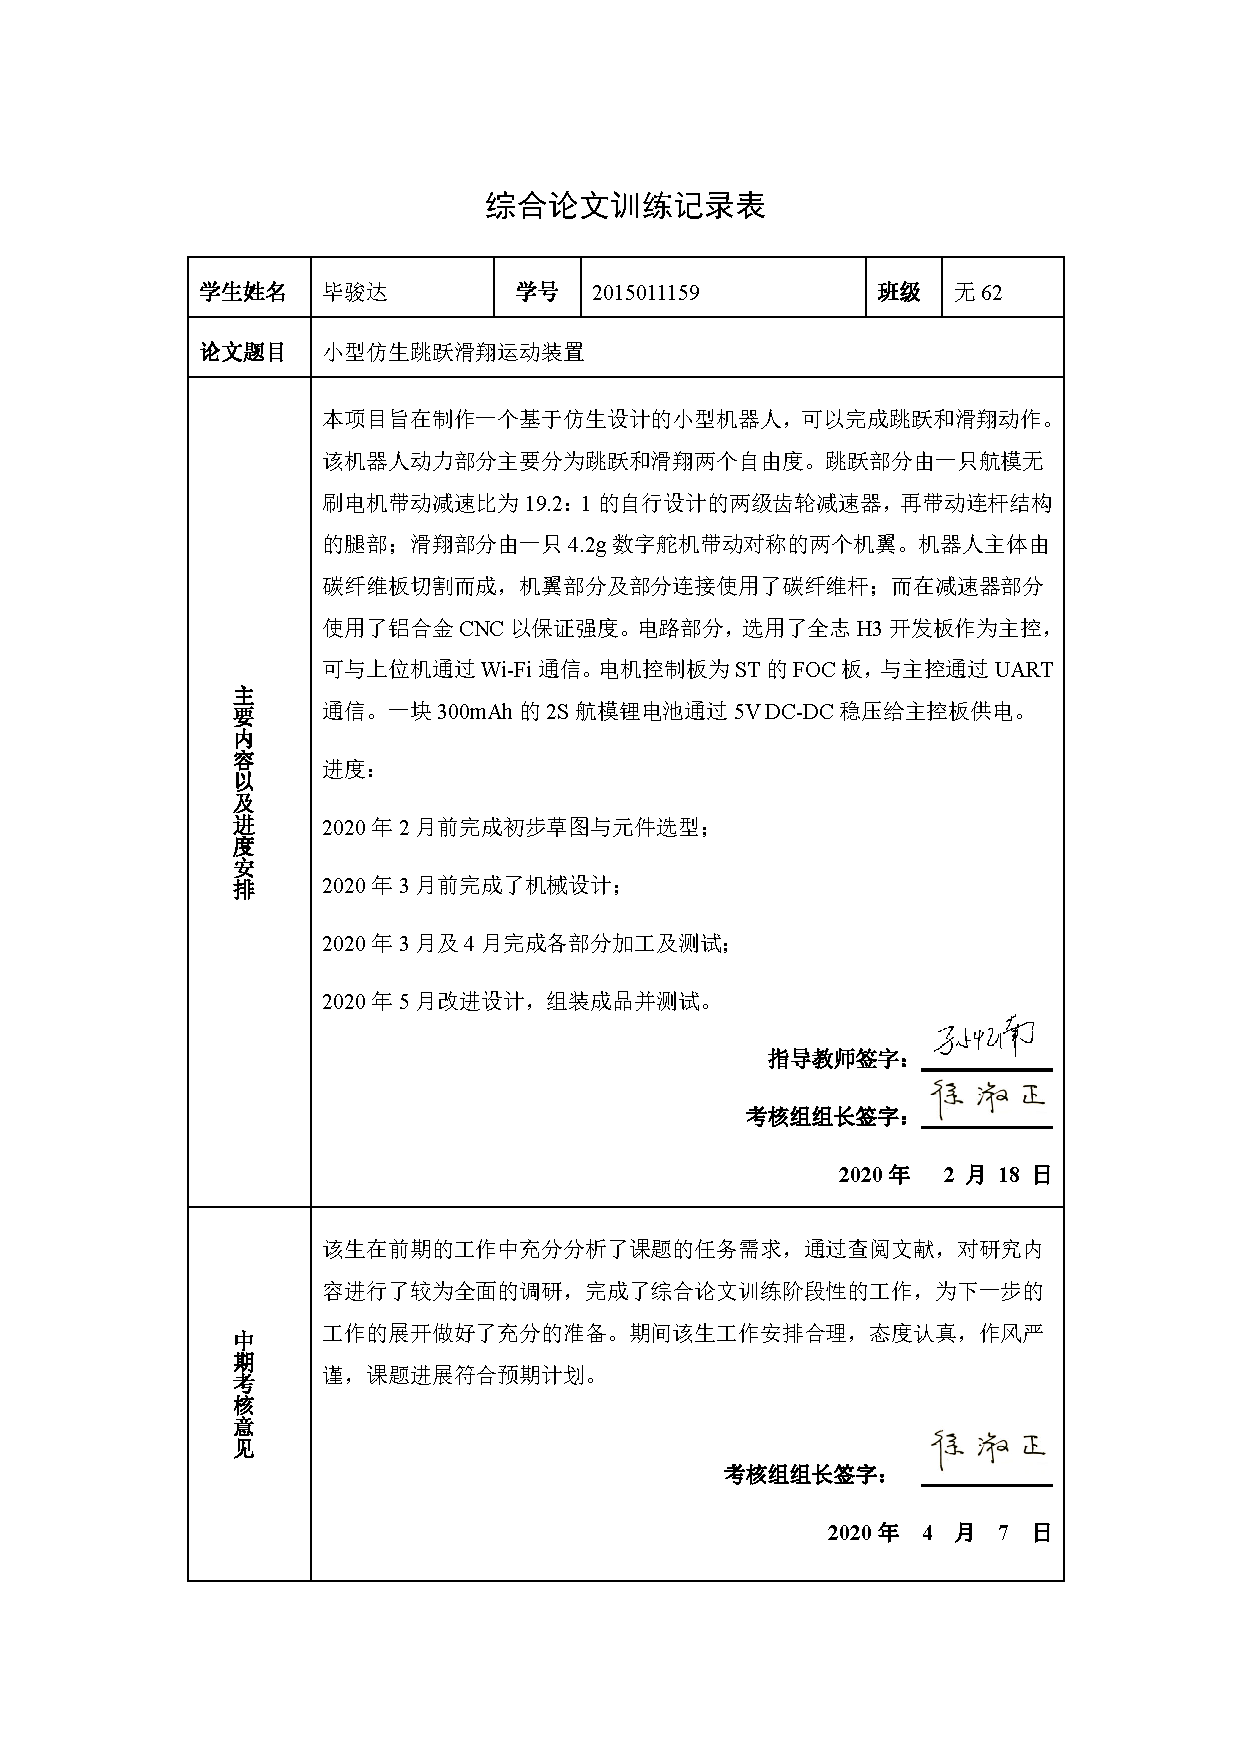
\includepdf[pages=-]{scan-record.pdf}

\end{document}
